\documentclass[11pt,a4paper]{article}
\usepackage[margin=2.3cm]{geometry}
\usepackage{amsmath,amssymb,bm}
\usepackage{graphicx}
\usepackage{booktabs}
\usepackage{longtable}
\usepackage{xcolor}
\usepackage[colorlinks=true,linkcolor=blue!50!black,citecolor=green!40!black,urlcolor=blue!60!black]{hyperref}
\numberwithin{equation}{section}
\graphicspath{{../figures/}}
\newcommand{\sq}{\sqrt{f_R}}
\newcommand{\dd}{\mathrm{d}}
\newcommand{\jh}{\hat\jmath_\ell}
\newcommand{\yh}{\hat y_\ell}

\title{Gravitational-wave perturbations of a spherical thin shell\\[2pt]
\large flat interior, Schwarzschild exterior: junction conditions, scattering coefficients\\ and quasinormal modes}
\author{Derivation document accompanying the code in \texttt{code/}}
\date{}

\begin{document}
\maketitle

\begin{abstract}
We derive, from first principles and with symbolic verification, the linearized Israel junction
conditions for odd- and even-parity gravitational perturbations of a spherical thin shell that separates
a flat interior from a Schwarzschild exterior, and use them to compute reflection/transmission
coefficients and quasinormal modes (QNMs). Two shell models are treated: a \emph{truly static} perfect-fluid
shell (model C) and a pure domain wall adiabatically frozen at its turning point (model A). The dust
shell proposed as ``Option B'' in the task statement does not exist as a static configuration, and we
show why. In the odd sector the junction conditions are model independent and of the scalar form
$[\Psi]=0$, $[\dd\Psi/\dd x]=\Delta\Psi$. In the even sector they form a frequency-dependent $2\times2$ transfer
matrix that involves the radial displacement of the shell and the motion of its matter. All results are
validated by independent numerical methods and against the literature. In particular we reproduce the
Schwarzschild QNMs and reflectivity, and the recent result of Pitre, Schneider \& Poisson (2026) that the
static fluid shell is dynamically unstable.
\end{abstract}

\tableofcontents

%======================================================================
\section*{Statement of the model and of the regime of validity}
\addcontentsline{toc}{section}{Statement of the model and of the regime of validity}
\begin{itemize}
\item \textbf{Model C (primary; truly static).} A perfect-fluid shell,
  $S^{ab}=\sigma u^au^b+p(h^{ab}+u^au^b)$, in \emph{exact} static equilibrium at areal radius $R>2M$, with
  $\sigma=(1-\sq)/(4\pi R)$ and $p=\sigma\kappa$, $\kappa=(1-\sq)/(4\sq)$ (Sec.~\ref{sec:bg}). In the
  language of Ipser \& Sikivie this is ``Option C'', $\tau/\sigma=-\kappa<0$, with $\kappa$ fixed by $R/M$.
  Perturbations of the shell matter obey a barotropic (polytropic) law
  $\delta p=\Gamma\, p\,\delta\sigma/(\sigma+p)$, and the fiducial adiabatic index is $\Gamma=2$. The
  background is exactly static. However, the configuration is \emph{linearly unstable} to even-parity
  nonradial perturbations. The growth rate is ${\rm Im}\,\omega\simeq0.5$--$0.7\,(M/R^3)^{1/2}$
  (Pitre, Schneider \& Poisson 2026 [PSP26]; reproduced in Sec.~\ref{sec:res-matter}).
\item \textbf{Model A (adiabatic).} A pure domain wall ($\tau=\sigma$, $S^{ab}=-\sigma h^{ab}$) frozen at
  its turning point $\dot R=0$, where $\ddot R=-(1+3\sq)/(2R)<0$. The background is \emph{not} static; it is
  momentarily static. The frozen-coefficient approximation is valid for $\omega\gg\omega_{\rm dyn}$, and
  the code quantifies its error. The constraint equations are violated at relative order
  $\omega_{\rm dyn}/\omega$ and energy conservation at order $(\omega_{\rm dyn}/\omega)^2$
  (Sec.~\ref{sec:evenA}).
\item \textbf{Odd parity.} The junction conditions are identical for both models, and indeed for any
  perfect-fluid shell with $\omega\neq0$ (Sec.~\ref{sec:odd}).
\item \textbf{Regime.} Real-frequency results (reflection/transmission) describe the static (C) or frozen
  (A) background. They are physically meaningful for $\omega$ well above the instability or collapse
  rates: $\omega\gg0.6(M/R^3)^{1/2}$ for C and $\omega\gg\omega_{\rm dyn}$ for A. Numerical values
  are given in Table~\ref{tab:bg}. QNMs are eigenvalues of the linearized problem about the stated
  background.
\end{itemize}
Units $G=c=1$. Frequencies are quoted as $\omega M$, the time dependence is $e^{-i\omega t}$, and $t$ is the
Schwarzschild (Killing) time of the exterior.

%======================================================================
\section{Background spacetime and shell; the collapse problem}\label{sec:bg}

\subsection{Thin-shell formalism}
Let $\Sigma$ be the timelike world-tube of the shell with intrinsic coordinates $y^a=(\tau,\theta,\phi)$,
tangent vectors $e^\alpha_a=\partial x^\alpha/\partial y^a$, and unit normal $n_\alpha$ pointing from the
interior ($-$) to the exterior ($+$). The induced metric and extrinsic curvature are
\begin{equation}
h_{ab}=g_{\alpha\beta}e^\alpha_ae^\beta_b,\qquad
K_{ab}=e^\alpha_ae^\beta_b\nabla_\alpha n_\beta=-n_\mu\left(\partial_ae^\mu_b+\Gamma^\mu_{\nu\rho}e^\nu_ae^\rho_b\right),
\label{eq:Kab}
\end{equation}
[Ipser \& Sikivie 1984 (IS84) Eqs.~(2.1)--(2.3); Poisson 2004 (P04) Secs.~3.1, 3.7]. The junction conditions
are the continuity of the induced metric and the Lanczos--Israel condition,
\begin{equation}
[h_{ab}]=0,\qquad [K_{ab}]-h_{ab}[K]=-8\pi S_{ab},\qquad [X]\equiv X|_{+}-X|_{-},
\label{eq:israel}
\end{equation}
(P04 Eqs.~3.49 and 3.56; IS84 Eq.~2.6). They imply the conservation law $D_bS^{ab}=0$ when the two sides are
vacuum (IS84 Eq.~2.8a).

\subsection{Spherical shell}
Birkhoff's theorem and regularity at $r=0$ fix the interior to be Minkowski
(\texttt{interior\_ondas\_cascara}, Sec.~1), $\dd s_-^2=-\dd T^2+\dd r^2+r^2\dd\Omega^2$. The exterior is
Schwarzschild, $\dd s_+^2=-f\dd t^2+f^{-1}\dd r^2+r^2\dd\Omega^2$ with $f=1-2M/r$ (IS84 Eq.~3.1). For a shell
$r=R(\tau)$ with $\alpha=(1+\dot R^2)^{1/2}$ and $\beta=(f(R)+\dot R^2)^{1/2}$ (IS84 Eq.~3.4), the
nonvanishing mixed components of the extrinsic curvature are (IS84 Eqs.~3.5--3.6; P04 Eq.~3.65)
\begin{equation}
K^\theta{}_\theta\big|_+=\frac{\beta}{R},\quad K^\theta{}_\theta\big|_-=\frac{\alpha}{R},\qquad
K^\tau{}_\tau\big|_+=\frac{\ddot R+M/R^2}{\beta},\quad K^\tau{}_\tau\big|_-=\frac{\ddot R}{\alpha}.
\label{eq:Kbg}
\end{equation}
With $S^a{}_b={\rm diag}(-\sigma,p,p)$, Eq.~\eqref{eq:israel} gives
\begin{equation}
\sigma=-\frac{1}{4\pi}[K^\theta{}_\theta]=\frac{\alpha-\beta}{4\pi R},\qquad
p=\frac{1}{8\pi}\left([K^\tau{}_\tau]+[K^\theta{}_\theta]\right).
\label{eq:sigp}
\end{equation}
These are equivalent to IS84's equations of motion, Eqs.~(3.7a,b), written with the tension $\tau=-p$:
\begin{equation}
(\alpha+\beta)\ddot R=-\frac{\alpha M}{R^2}-\frac{2\tau}{\sigma}\frac{\alpha\beta(\alpha+\beta)}{R},\qquad
(\alpha-\beta)\ddot R=-\frac{\alpha M}{R^2}+4\pi(\sigma-2\tau)\alpha\beta .
\label{eq:IS37}
\end{equation}
Squaring the first of Eqs.~\eqref{eq:sigp} gives the mass formula $M=\tfrac12(\alpha+\beta)4\pi\sigma R^2$
(IS84 Eq.~3.8). At a moment with $\dot R=0$ this becomes
\begin{equation}
4\pi\sigma R=1-\sq,\qquad\text{equivalently}\qquad M=4\pi\sigma R^2(1-2\pi\sigma R),
\label{eq:IS39}
\end{equation}
which is IS84 Eq.~(3.9). The code checks it to machine precision (Table~\ref{tab:bg}). Here and below
$f_R\equiv f(R)$.

\subsection{The collapse problem and the choice of shell model}\label{sec:choice}
Setting $\dot R=\ddot R=0$ in Eq.~\eqref{eq:IS37} requires
\begin{equation}
\frac{M}{R^2}+\frac{2\tau}{\sigma}\frac{f_R+\sq}{R}=0\quad\Longrightarrow\quad
\frac{\tau}{\sigma}=-\kappa,\qquad \kappa=\frac{M}{2R\sq(1+\sq)}=\frac{1-\sq}{4\sq}>0 .
\label{eq:kappa}
\end{equation}
A static shell therefore needs \emph{negative tension}, i.e.\ positive surface pressure $p=\kappa\sigma$.
This reproduces P04 Eq.~(3.81), $p=(1-M/R-\sq)/(8\pi R\sq)$. We now evaluate the options listed in the
task.

\paragraph{Option B (static dust shell) does not exist.}
For dust, $\tau=0$, and the first of Eqs.~\eqref{eq:IS37} gives $(\alpha+\beta)\ddot R=-\alpha M/R^2<0$ for
any $\dot R$. As IS84 state after their Eq.~(3.7a), \emph{``$\ddot R$ is always negative if $\tau\ge0$''}. The
same conclusion follows from P04 Eq.~(3.70), $M=m(1+\dot R^2)^{1/2}-m^2/2R$ with $m=4\pi\sigma R^2$
conserved: a dust shell can only be \emph{momentarily} static, at the turning point. There it obeys the same
relation \eqref{eq:IS39} as the domain wall, and $\ddot R=-M/[R^2(1+\sq)]$. The formula
$M=4\pi\sigma R^2\sq$ quoted in the task statement does not follow from the junction conditions. It coincides
with neither $M=4\pi\sigma R^2(1-2\pi\sigma R)$ nor the static relation $4\pi\sigma R=1-\sq$. We therefore
do not implement Option B.

\paragraph{Option C (static fluid shell): chosen as primary model (model C).}
Equation~\eqref{eq:kappa} shows that $\kappa$ is \emph{not} a free parameter: for static equilibrium it is
fixed by $R/M$ (Table~\ref{tab:bg}). The family is parametrized by compactness. The dominant energy condition
$p\le\sigma$ requires $\kappa\le1$, i.e.\ $\sq\ge1/5$ or $R\ge25M/12\simeq2.083M$. For perturbations one must
also specify how the shell's pressure responds, $\delta p=v_s^2\delta\sigma$. We use the polytropic law of
PSP26 (their Eqs.~1.1, 2.5--2.6), $\delta p=\Gamma p/(\sigma+p)\,\delta\sigma$, i.e.
$v_s^2=\Gamma\kappa/(1+\kappa)$, with fiducial $\Gamma=2$. Our $\sigma$ is PSP26's energy density $\mu$.
Causality $v_s^2\le1$ holds for $\Gamma=2$ iff $\kappa\le1$. Our model-C results are therefore restricted to
$R\ge2.1M$, except where stated.

\paragraph{Option A (domain wall, adiabatic): implemented as model A.}
For $\tau=\sigma$ and $\dot R=0$, Eqs.~\eqref{eq:Kbg}--\eqref{eq:sigp} give $[K^\tau{}_\tau]=[K^\theta{}_\theta]=-4\pi\sigma$,
and hence
\begin{equation}
\ddot R=-\frac{M}{R^2(1+\sq)}-\frac{2\sq}{R}=-\frac{1+3\sq}{2R}\qquad(\text{proper time}).
\label{eq:Rdd}
\end{equation}
The first form is IS84 Eq.~(3.7a) with $\alpha=1$, $\beta=\sq$. The symbolic derivation obtains the same
$\ddot R$ independently, from the angular Israel equation at the frozen instant. The background is
momentarily static. We define the dynamical frequency in exterior time as
$\omega_{\rm dyn}=\sq\,(|\ddot R|/R)^{1/2}$; the frozen approximation requires $\omega\gg\omega_{\rm dyn}$.

\paragraph{Option D (Schwarzschild/de Sitter interior).} Not implemented. It changes the interior problem,
and Pani et al.\ (2009) have treated its de Sitter version. Our model C is the $\Sigma\neq0$,
Minkowski-interior member of the same family of thin-shell ``gravastars''.

\paragraph{Why both static options end up dynamical.}
Model A collapses on the timescale $\omega_{\rm dyn}^{-1}$. Model C has an exact static background, but it
possesses an unstable even-parity ``matter mode''. PSP26 found this mode, and we find it independently
(Sec.~\ref{sec:res-matter}), with growth rate $\simeq0.6(M/R^3)^{1/2}$. In both cases real-frequency
scattering is an idealization valid for $\omega$ large compared with these rates. Wave-mode QNMs have
$\omega\sim1/R$, which is larger than $(M/R^3)^{1/2}$ for all $R>2M$ by a factor $(R/M)^{1/2}$.

\subsection{Time normalization: interior blueshift}\label{sec:blueshift}
Continuity of $h_{ab}$ at a static shell requires $\dd T=\sq\,\dd t$ (P04 Eq.~3.75). A monochromatic
perturbation $e^{-i\omega t}$ outside is therefore $e^{-i\nu T}$ inside, with
\begin{equation}
\nu=\frac{\omega}{\sq} .
\label{eq:nu}
\end{equation}
The regular interior solution is $\jh(\nu r)$, not $\jh(\omega r)$ as written in the prior notes and in the task
statement. This is essential near $R\to2M$, where $\nu\gg\omega$. PSP26 (their $w=F^{-1/2}\omega$) adopt the
same normalization. It is convenient to define a \emph{global tortoise coordinate}
\begin{equation}
x=r_*=r+2M\ln(r/2M-1)\ \ (r>R),\qquad x=r_*(R)+(r-R)/\sq\ \ (r<R),
\label{eq:x}
\end{equation}
in which both sides obey $-\partial_t^2\Psi+\partial_x^2\Psi-V\Psi=0$, with $V_{\rm int}=f_R\,\ell(\ell+1)/r^2$
(Fig.~\ref{fig:pot}).

\begin{table}[t]\centering
\caption{Background quantities (from \texttt{results/validation.json}). The column
$(M/R^3)^{1/2}$ sets the scale of the model-C instability rate ($\simeq0.6$ times this) and of the
matter modes. $\omega_{\rm dyn}$ is the domain-wall collapse rate in exterior time.}\label{tab:bg}
\begin{tabular}{rrrrrrrrr}\toprule
$R/M$ & $\sigma M$ & $pM$ & $\kappa=p/\sigma$ & $v_s^2(\Gamma{=}2)$ & I\&S (3.7a) resid. & $\ddot R_{\rm wall}M$ & $\omega_{\rm dyn}M$ & $(M/R^3)^{1/2}M$\\\midrule
2.2 & 0.02527 & 1.463e-02 & 0.5792 & 0.7335 & 0.00e+00 & -0.4328 & 0.1337 & 0.3065 \\
3.0 & 0.01121 & 2.052e-03 & 0.1830 & 0.3094 & 1.39e-17 & -0.4553 & 0.2249 & 0.1925 \\
6.0 & 0.00243 & 1.367e-04 & 0.0562 & 0.1064 & 0.00e+00 & -0.2875 & 0.1787 & 0.0680 \\
10.0 & 0.00084 & 2.479e-05 & 0.0295 & 0.0573 & 1.73e-18 & -0.1842 & 0.1214 & 0.0316 \\
\bottomrule\end{tabular}

\end{table}

\begin{figure}[t]\centering
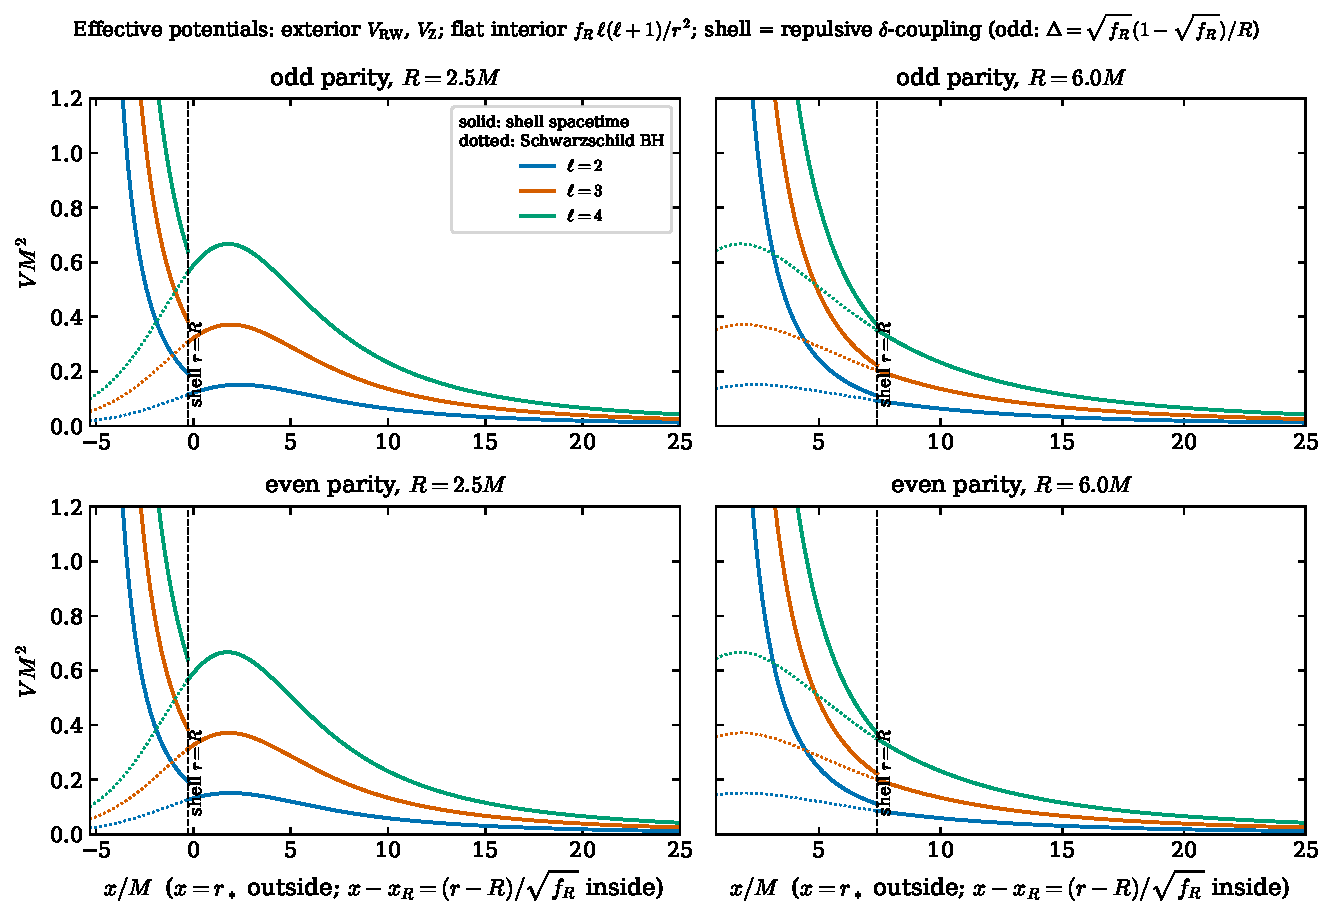
\includegraphics[width=\textwidth]{fig01_potentials.pdf}
\caption{Effective potentials in the global tortoise coordinate \eqref{eq:x} for $\ell=2,3,4$. Outside:
$V_{\rm RW}$ (RW57 Eq.~25; MP05 Eq.~5.15) and $V_{\rm Z}$ (Zerilli 1970 Eq.~5; MP05 Eq.~4.26). Inside:
$f_R\,\ell(\ell+1)/r^2$. Dotted lines show the Schwarzschild continuation to the horizon. The odd-parity shell
adds a repulsive $\delta$-function of strength $\Delta_{\rm odd}$, Eq.~\eqref{eq:oddfinal}. The even-parity
coupling is a frequency-dependent $2\times2$ matrix.}\label{fig:pot}
\end{figure}


%======================================================================
\section{Perturbation equations}\label{sec:pert}
We follow Martel \& Poisson (2005) [MP05] throughout. Spherical-harmonic labels are omitted. The odd-parity
harmonics are $X_A=-\varepsilon_A{}^BD_BY$ and $X_{AB}=-\tfrac12(\varepsilon_A{}^CD_B+\varepsilon_B{}^CD_A)D_CY$
(MP05 Eqs.~3.2, 3.7). The even-parity ones are $Y_A=D_AY$ and $Y_{AB}=[D_AD_B+\tfrac12\ell(\ell+1)\Omega_{AB}]Y$
(MP05 Eqs.~3.1, 3.6). We use $\lambda=\ell(\ell+1)$ and $\mu=(\ell-1)(\ell+2)$, and Regge--Wheeler (RW) gauge on
each side: $h_2=0$ (odd) and $j_a=G=0$ (even) (MP05 Secs.~IV.A, V.A).

\subsection{Exterior (Schwarzschild)}
\paragraph{Odd parity.} $p_{aB}=h_aX_B$ with $h_a=(h_t,h_r)$ (MP05 Eq.~5.2). The Cunningham--Price--Moncrief
function
\begin{equation}
\Psi_{\rm odd}=\frac{2r}{\mu}\,\varepsilon^{ab}\Big(\partial_ah_b-\frac2r r_ah_b\Big)
=\frac{2r}{\mu}\Big(\partial_rh_t-\partial_th_r-\frac2rh_t\Big)
\label{eq:cpm}
\end{equation}
(MP05 Eq.~5.13, with $\varepsilon_{tr}=1$) obeys the Regge--Wheeler equation (MP05 Eqs.~5.14--5.15; RW57 Eq.~25)
\begin{equation}
\frac{\dd^2\Psi}{\dd r_*^2}+\big[\omega^2-V_{\rm RW}(r)\big]\Psi=0,\qquad
V_{\rm RW}=f\Big[\frac{\lambda}{r^2}-\frac{6M}{r^3}\Big].
\label{eq:RW}
\end{equation}
The vacuum field equations, MP05 Eqs.~(5.8), (5.9), (5.18), can be inverted as
\begin{equation}
h_t=\frac f2\,\partial_r(r\Psi_{\rm odd}),\qquad h_r=\frac{r}{2f}\partial_t\Psi_{\rm odd}=-\frac{i\omega r}{2f}\Psi_{\rm odd}.
\label{eq:oddrecon}
\end{equation}
The second relation is MP05 Eq.~(5.18), $\Psi_{\rm RW}=r^ah_a/r=\tfrac12\partial_t\Psi_{\rm odd}$, in vacuum. The
first follows from $P=\nabla_ah^a=0$ (MP05 Eq.~5.9). \emph{Verification:}
\texttt{symbolic/vacuum\_relations.py} linearizes the Einstein tensor by brute force for a generic
axisymmetric harmonic, keeping $\lambda$ symbolic. It checks that Eqs.~\eqref{eq:oddrecon} satisfy all
odd-parity field equations identically when $\Psi$ obeys \eqref{eq:RW}, and that \eqref{eq:cpm} reproduces
$\Psi$ (log in \texttt{results/log\_vacuum\_relations.txt}).

\paragraph{Even parity.} $p_{ab}=h_{ab}Y$ with $h_{tt}=fH_0$, $h_{tr}=H_1$, $h_{rr}=H_2/f$, and
$p_{AB}=r^2K\Omega_{AB}Y$ (MP05 Eqs.~4.1--4.3). The trace-free angular equation gives $H_0=H_2\equiv H$. The
Zerilli--Moncrief function (MP05 Eqs.~4.23--4.24)
\begin{equation}
\Psi_{\rm even}=\frac{2r}{\lambda}\Big[K+\frac{2}{\Lambda}\big(r^ar^bh_{ab}-r\,r^a\nabla_aK\big)\Big]
=\frac{2r}{\lambda}\Big[K+\frac{2f}{\Lambda}\big(H-rK'\big)\Big],\qquad\Lambda=\mu+\frac{6M}{r},
\label{eq:zm}
\end{equation}
obeys the Zerilli equation, i.e.\ Eq.~\eqref{eq:RW} with $V_{\rm RW}\to V_{\rm Z}$,
\begin{equation}
V_{\rm Z}=f\,\frac{2n^2(n+1)r^3+6n^2Mr^2+18nM^2r+18M^3}{r^3(nr+3M)^2},\qquad n=\frac{\mu}{2},
\label{eq:VZ}
\end{equation}
(Zerilli 1970 Eq.~5). This equals $f$ times MP05 Eq.~(4.26); the identity is checked symbolically. The code
derives the first-order system (the $tr$, $t\theta$ and $r\theta$ components of the linearized Einstein
equations; it agrees with Zerilli 1970's system) and the algebraic identity (from $G_{rr}$). It then inverts
\eqref{eq:zm} and obtains the reconstruction
\begin{align}
K&=f\,\Psi'+\frac{\mu(\mu+2)r^2+6\mu Mr+24M^2}{2r^2(\mu r+6M)}\,\Psi,\label{eq:Krec}\\
H_1&=-i\omega\Big[r\,\Psi'+\frac{\mu r^2-3\mu Mr-6M^2}{(r-2M)(\mu r+6M)}\,\Psi\Big],\label{eq:H1rec}\\
H&=f\,\frac{\mu r^2-3\mu Mr-6M^2}{(r-2M)(\mu r+6M)}\,\Psi'
+\Big[\frac{Q(r)}{2r^2(r-2M)(\mu r+6M)^2}-\frac{\omega^2r}{f}\Big]\Psi,\label{eq:Hrec}\\
Q(r)&=\mu^2(\mu+2)r^4-2M\mu^2(\mu-1)r^3-12M^2\mu(\mu-3)r^2-72M^3(\mu-1)r-144M^4,\nonumber
\end{align}
where $'=\dd/\dd r$. Substituting \eqref{eq:Krec}--\eqref{eq:Hrec} into all six independent linearized Einstein
equations gives zero identically once $\Psi$ obeys the Zerilli equation. The check is done exactly, in
rational arithmetic, at random rational values of $(r,M,\omega,\lambda)$. Substituting them into
\eqref{eq:zm} returns $\Psi$.

\paragraph{Chandrasekhar transformation.} The map
$Z=[\mu(\mu+2)+72M^2f/(r(\mu r+6M))]\Psi_{\rm RW}+12M\,\dd\Psi_{\rm RW}/\dd r_*$ (Chandrasekhar 1983,
Sec.~4.26; used by Pani et al.\ 2009 Sec.~III.B) takes RW solutions into Zerilli solutions for all $\omega$. It
is verified symbolically in \texttt{symbolic/exterior\_series.py}. Outgoing solutions map to outgoing ones,
with amplitude factor $\mu(\mu+2)+12iM\omega$.

\subsection{Interior (Minkowski)}
With $M=0$ both potentials reduce to $\lambda/r^2$, so both master functions obey
(\texttt{interior\_ondas\_cascara} Eqs.~6--9)
\begin{equation}
\Psi''+\Big[\nu^2-\frac{\lambda}{r^2}\Big]\Psi=0\qquad(0<r<R),
\label{eq:int}
\end{equation}
with $\nu$ the interior-time frequency \eqref{eq:nu}. The reconstruction formulas above hold with $M=0$ and
$\omega\to\nu$, since the interior is written in its own Minkowski time $T$.

%======================================================================
\section{Interior solution}\label{sec:interior}
The Riccati--Bessel functions $\jh(z)=zj_\ell(z)$ and $\yh(z)=zy_\ell(z)$ (Abramowitz \& Stegun 1972
Sec.~10.3; \texttt{interior\_ondas\_cascara} Eqs.~10, 26) solve \eqref{eq:int} with $z=\nu r$. Only
\begin{equation}
\Psi_{\rm int}=A\,\jh(\nu r),\qquad \jh(z)\to\frac{z^{\ell+1}}{(2\ell+1)!!}\ (z\to0),
\label{eq:intsol}
\end{equation}
is regular at the centre (\texttt{interior\_ondas\_cascara} Eqs.~11--13). The two parities share this profile;
they differ only through the junction conditions. For the \emph{open-interior} scattering problem
(Sec.~\ref{sec:RTdef}) we also use the Riccati--Hankel functions (e$^{-i\omega t}$ convention)
\begin{equation}
\hat h^{\rm out}_\ell=-\yh+i\jh\sim e^{+i(z-\ell\pi/2)},\qquad \hat h^{\rm in}_\ell=-\yh-i\jh\sim e^{-i(z-\ell\pi/2)},
\label{eq:hankel}
\end{equation}
with Wronskian $\jh\yh'-\jh'\yh=1$ (DLMF 10.50.1), so that ${\rm Im}(\hat h^{\rm in*}\hat h^{\rm in\,\prime})=-1$
exactly. The code evaluates $\jh$ both through \texttt{scipy.special.spherical\_jn} (complex argument) and by
direct DOP853 integration of \eqref{eq:int} from a power-series start. The two agree to $10^{-10}$
(\texttt{interior.regular\_numerical}).

%======================================================================
\section{Junction conditions}\label{sec:junction}

\subsection{Linearized matching: method}\label{sec:jmethod}
The perturbed metric on each side is written in that side's own RW gauge. RW gauge fixes the bulk gauge
freedom completely for $\ell\ge2$, but it is not adapted to the shell. The shell's world-tube is therefore
described on each side by a perturbed embedding (cf.\ Pani et al.\ 2009 Sec.~III.C and App.~A)
\begin{equation}
x^\mu_\pm(y)=X^\mu_{0\pm}(y)+\epsilon\,Z^\mu_\pm(y),\qquad
Z_+=(0,\ \xi_+Y,\ 0,\ 0),\qquad Z_-=(\zeta Y,\ \xi_-Y,\ \eta\,\partial_\theta Y,\ 0)\ [+\ \chi X^\phi\ \text{(odd)}],
\label{eq:embed}
\end{equation}
where $y^a=(\tau,\theta,\phi)$ are chosen to coincide with the exterior ones. $\xi_\pm$ are the radial
displacements of the shell in the two RW gauges. $\zeta$, $\eta$ ($\chi$) describe the relative
time/angular identification (twist) of the two sides. The unit normal is solved to first order from
$n_\mu e^\mu_a=0$ and $g^{\mu\nu}n_\mu n_\nu=1$. The induced metric and \eqref{eq:Kab} are then expanded to
$O(\epsilon)$ by brute force, including the displacement of the background fields,
$Q(X_0+\epsilon Z)=Q(X_0)+\epsilon Z^\mu\partial_\mu Q$. The result is projected on harmonics. The bulk
metric functions are replaced by the master functions through Eqs.~\eqref{eq:oddrecon} and
\eqref{eq:Krec}--\eqref{eq:Hrec}. The matter of the shell is perturbed as
$\sigma\to\sigma+\delta\sigma\,Y$, $p\to p+v_s^2\delta\sigma\,Y$, $u_A=U D_AY$ (even) or $U X_A$ (odd). For the
domain wall, $S_{ab}=-\sigma h_{ab}$ with $\sigma$ constant (IS84 Eq.~2.12). The equations \eqref{eq:israel}
become a linear system,
\begin{equation}
\mathsf A(\omega)\,\bm x=\mathsf B(\omega)\binom{\Psi_-(R)}{\Psi_-'(R)},\qquad
\bm x=(\text{shell variables},\ \Psi_+(R),\ \Psi_+'(R)),
\label{eq:linsys}
\end{equation}
whose last two components define the transfer matrix $\mathsf T$:
$(\Psi_+,\Psi_+')^{\rm T}=\mathsf T(\Psi_-,\Psi_-')^{\rm T}$. The whole construction is implemented in
\texttt{symbolic/derive\_junction.py}. That script also verifies the background Israel equations: they
vanish identically for Poisson's $\sigma$, $p$ and yield Eq.~\eqref{eq:Rdd} for the wall. It exports the
exact matrices $\mathsf A$, $\mathsf B$ as the Python modules \texttt{shellgw/junction\_\{odd,even\}\_\{A,C\}.py}.

\subsection{Odd parity: analytic derivation}\label{sec:odd}
Odd perturbations do not move the shell radially. $e_a$ and the normal are unperturbed except for the twist
$\chi$, and $n_\alpha=f^{-1/2}\partial_\alpha r$ remains exact to first order because $g^{rr}$ is not perturbed.
From \eqref{eq:Kab}, $K_{ab}=-N\Gamma^r{}_{ab}$ with $N=f^{-1/2}$. The first-order Christoffel symbols
$\delta\Gamma^r{}_{tA}=\tfrac f2(\partial_th_r-\partial_rh_t)X_A$ and $\delta\Gamma^r{}_{AB}=f h_r X_{AB}$ then give
\begin{equation}
\delta K_{tA}=\frac{\sqrt f}{2}\big(\partial_rh_t-\partial_th_r\big)X_A,\qquad
\delta K_{AB}=-\sqrt f\,h_r\,X_{AB}.
\label{eq:dKodd}
\end{equation}
The first is Eq.~(12) of \texttt{burbuja\_matching\_israel}. With Eq.~\eqref{eq:cpm},
$\partial_rh_t-\partial_th_r=\mu\Psi/(2r)+2h_t/r$. We convert to proper time on $\Sigma$
($e_\tau=f_R^{-1/2}\partial_t$ outside, $\partial_T$ inside) and define the common quantity
$\mathcal H\equiv\delta h_{\tau A}$, the coefficient of $X_A$. Then
\begin{equation}
\text{outside:}\quad \mathcal H=\frac{h_t^+}{\sq},\quad \delta K^+_{\tau A}=\frac{\mu\Psi_+}{4R}+\frac{\sq\,\mathcal H}{R};\qquad
\text{inside:}\quad \mathcal H=h_T^-,\quad \delta K^-_{\tau A}=\frac{\mu\Psi_-}{4R}+\frac{\mathcal H}{R}.
\label{eq:oddside}
\end{equation}
Continuity of $\delta h_{\tau A}$ is built in by using the single symbol $\mathcal H$. Continuity of
$\delta h_{AB}$ is automatic, since $h_2=0$ on both sides and hence $\chi=0$. Three equations remain:
\begin{enumerate}
\item The \emph{$AB$ Israel equation.} Since $\delta h_{AB}=0$ and $u_Au_B=O(\epsilon^2)$,
  $\delta S_{AB}^{\rm odd}=0$, and so $[\sqrt f h_r]=0$. With \eqref{eq:oddrecon} on each side
  ($h_r^-=-i\nu R\Psi_-/2$), this gives exactly
  \begin{equation}\Psi_+(R)=\Psi_-(R).\label{eq:oddJ1}\end{equation}
\item The \emph{$\tau A$ Israel equation.} With $\delta S_{\tau A}=-(\sigma+p)U+p\,\mathcal H$ and the trace of
  \eqref{eq:israel}, $[K]=4\pi(2p-\sigma)$, we get
  $[\delta K_{\tau A}]=-4\pi\sigma\mathcal H+8\pi(\sigma+p)U$. By \eqref{eq:oddside} the left side equals
  $\mu[\Psi]/(4R)+(\sq-1)\mathcal H/R$, and $(\sq-1)/R=-4\pi\sigma$. Hence
  $\mu[\Psi]/(4R)=8\pi(\sigma+p)U$, and with \eqref{eq:oddJ1}, $U=0$: the shell matter does not move.
  This is consistent with the odd part of $D_bS^{ab}=0$, which gives $\partial_\tau(u_A)=0$, hence $U=0$ for
  $\omega\neq0$. The background trace $[K]^{(0)}$ identified as ``the remaining step'' in
  \texttt{burbuja\_matching\_israel} Eq.~(13) combines with $\delta S_{\tau A}$ into
  $[K]^{(0)}-8\pi p=-4\pi\sigma$. The $p$ dependence, and with it the $\ddot R$ dependence of the domain wall,
  \emph{cancels identically}.
\item \emph{Continuity of $\mathcal H$.} From \eqref{eq:oddrecon},
  $\mathcal H=\tfrac12(r\Psi_-)'|_R=\tfrac{\sq}{2}(r\Psi_+)'|_R$.
\end{enumerate}
With \eqref{eq:oddJ1}, item 3 gives
\begin{equation}
\boxed{\ \Psi_+=\Psi_-,\qquad \sq\,\Psi_+'-\Psi_-'=\frac{1-\sq}{R}\,\Psi=4\pi\sigma\,\Psi\ }
\qquad\Longleftrightarrow\qquad
\Big[\frac{\dd\Psi}{\dd\ell}\Big]=4\pi\sigma\Psi,
\label{eq:oddfinal}
\end{equation}
with $\ell$ the proper radial distance. In the global tortoise coordinate \eqref{eq:x},
$[\dd\Psi/\dd x]=\Delta_{\rm odd}\Psi$ with
\begin{equation}
\Delta_{\rm odd}=\frac{\sq(1-\sq)}{R}=4\pi\sigma\sq>0 ,
\label{eq:Deltaodd}
\end{equation}
i.e.\ the shell acts as a \emph{repulsive $\delta$-function potential} $\Delta_{\rm odd}\,\delta(x-x_R)$. This is
precisely the schematic form anticipated in the task, with $\Delta$ independent of $\omega$ and of the shell's
equation of state. The transfer matrix is
$\mathsf T_{\rm odd}=\begin{pmatrix}1&0\\ (1-\sq)/(R\sq) & 1/\sq\end{pmatrix}$, and $\det\mathsf T_{\rm odd}=f_R^{-1/2}$
(flux conservation, Sec.~\ref{sec:RTdef}).

\emph{Checks.} (i) The brute-force symbolic derivation, with the twist $\chi$ and the velocity $U$ kept as
unknowns, reproduces \eqref{eq:oddfinal} for model C (4 equations, 4 unknowns, $\chi=U=0$) and model A.
For model A the system is overdetermined (4 equations, 3 unknowns) but consistent, with rank 3; the
difference between the two models' transfer matrices is $10^{-15}$. (ii) \eqref{eq:oddfinal} agrees with
PSP26 Eq.~(5.23)/(97), $F^{1/2}\eta_{\rm out}-\eta_{\rm in}+F^{1/2}-1=0$ with $\eta=R\psi'/\psi$. The phase
factors of their retarded-time slicing cancel because $w=F^{-1/2}\omega$. (iii) It agrees with Pani et al.\
(2009) Eqs.~(3.29) and (A35), $[h_0]=0$ and $[\sqrt h\,h_1]=0$. In their $\Sigma=0$ model $h$ is continuous
and \(\Psi\), \(\Psi'\) are continuous; for $\Sigma\neq0$ their Regge--Wheeler function $\Psi_{\rm RW}\propto\sqrt h\,h_1$
jumps, whereas the CPM function \eqref{eq:cpm} is continuous. (iv) As $M\to0$ ($\sigma\to0$), $\mathsf T\to\mathbb{I}$:
the inviscid/transparent limit of Boyanov et al.\ (2024), continuity of $\Psi$ and $\Psi'$.



\subsection{Even parity}\label{sec:even}
\paragraph{Induced metric.} The first-order induced metric computed from the two sides is
(harmonic coefficients of $Y$, $D_AY$, $\Omega_{AB}Y$ and $Y_{AB}$)
\begin{align}
\text{outside:}&\quad \delta h_{\tau\tau}=H_+-\frac{2M}{R(R-2M)}\xi_+,\quad \delta h_{\tau A}=0,\quad
\delta h^{\rm tr}_{AB}=R^2K_++2R\xi_+,\quad \delta h^{\rm tf}_{AB}=0,\nonumber\\
\text{inside:}&\quad \delta h_{\tau\tau}=H_-+2i\nu\zeta,\quad \delta h_{\tau A}=-\zeta-i\nu R^2\eta,\quad
\delta h^{\rm tr}_{AB}=R^2K_--\lambda R^2\eta+2R\xi_-,\quad \delta h^{\rm tf}_{AB}=2R^2\eta .
\label{eq:dheven}
\end{align}
The first junction condition therefore forces $\eta=\zeta=0$ (no relative twist of the two identifications)
and leaves
\begin{equation}
H_+-\frac{2M}{R(R-2M)}\,\xi_+=H_-,\qquad RK_++2\xi_+=RK_-+2\xi_- .
\label{eq:evencont}
\end{equation}
These agree with Pani et al.\ (2009) Eqs.~(A16) and (A20), $[[2hz+aK]]=0$ and $[[x]]=[[w]]=[[y]]=0$. The radial
displacement of the shell differs between the two RW gauges ($\xi_+\neq\xi_-$). This is why the even sector
cannot be reduced to a scalar jump condition.

\paragraph{Israel equations.} The four even components ($\tau\tau$, $\tau A$, trace and trace-free $AB$) of
$[\delta K_{ab}-\delta h_{ab}K-h_{ab}\delta K]=-8\pi\delta S_{ab}$ involve
$(H_\pm,H_\pm',K_\pm,K_\pm',H_{1\pm},\xi_\pm)$ and the matter variables. For model C,
\begin{equation}
\delta S_{\tau\tau}=\delta\sigma-\sigma\,\delta h_{\tau\tau},\quad
\delta S_{\tau A}=-(\sigma+p)U+p\,\delta h_{\tau A},\quad
\delta S^{\rm tr}_{AB}=v_s^2\delta\sigma R^2+p\,\delta h^{\rm tr}_{AB},\quad
\delta S^{\rm tf}_{AB}=p\,\delta h^{\rm tf}_{AB}.
\label{eq:dSeven}
\end{equation}
For model A, $\delta S_{ab}=-\sigma\delta h_{ab}$. With Eqs.~\eqref{eq:Krec}--\eqref{eq:Hrec} on each side
($M\to0$, $\omega\to\nu$ inside), the system \eqref{eq:linsys} has the following size.
\begin{itemize}
\item Model C: 8 equations for the 8 unknowns $(\xi_+,\xi_-,\zeta,\eta,\delta\sigma,U,\Psi_+,\Psi_+')$. It has
full rank, and its solution defines $\mathsf T_{\rm even}^{\rm C}(\omega;\ell,R/M,\Gamma)$.
\item Model A: 8 equations for 6 unknowns (no matter variables). See below.
\end{itemize}
The individual first-order extrinsic-curvature components are lengthy. They are generated and stored
exactly by \texttt{symbolic/derive\_junction.py} and exported to \texttt{shellgw/junction\_even\_\{C,A\}.py}.

\paragraph{Structure of the result.} In contrast to odd parity,
\begin{itemize}
\item $\Psi$ is \emph{discontinuous}. $\mathsf T_{\rm even}$ is a full $2\times2$ matrix that depends on
frequency (through $\omega^2$ terms in $H$ and through the shell's inertia) and on the shell equation of state
through $v_s^2$. The schematic form $[\Psi]=0$, $[\partial_x\Psi]=\Delta\Psi$ does \emph{not} hold. As
anticipated in the task, the even problem is a genuine $2\times2$ matching, with the shell's radial motion
$\xi_\pm$ and its density and velocity perturbations eliminated.
\item $\det\mathsf T^{\rm C}_{\rm even}=f_R^{-1/2}$ exactly. In the code this holds to $10^{-12}$ in double
precision and $10^{-15}$ in 40-digit arithmetic, for all $\omega$, $\ell$, $R$ and $\Gamma$ tested. For real
$\omega$ the matrix conserves the flux $J$, so $\mathcal R+\mathcal T=1$ (Sec.~\ref{sec:res-valid}).
\item Transparent limit: $\mathsf T_{\rm even}\to\mathbb{I}$ as $M\to0$ at fixed $R$ (i.e.\ $\sigma,p\to0$), for both
models, to $4\times10^{-9}$ at $M=10^{-8}$.
\item The matrix has poles at the frequencies of the \emph{matter modes} of the shell, which are absent in
odd parity. For model C their QNM counterparts, including a purely imaginary unstable mode, reproduce PSP26
quantitatively (Sec.~\ref{sec:res-matter}).
\end{itemize}

\paragraph{Model A: an adiabatic, not exact, matching.}\label{sec:evenA}
For an exact solution of the moving-shell problem, the $\tau\tau$ and $\tau A$ Israel equations follow from
the others by the Codazzi identity $D_b([K^b{}_a]-\delta^b_a[K])=0$ together with $D_bS^{ab}=0$. Accordingly, the
odd-parity model-A system, although overdetermined, is exactly consistent. In the even sector the frozen,
monochromatic ansatz is \emph{not} an exact solution at the turning point, because
$\dddot T_0\propto\ddot R^2\neq0$ there even though $\dot R=\ddot T_0=0$. The two constraint rows are then
violated. Indeed ${\rm rank}\,\mathsf A=6$ while ${\rm rank}[\mathsf A|\mathsf B]=8$. We solve the six
evolution equations (continuity and angular Israel equations) and monitor the constraints. Their relative
violation decreases as $\omega_{\rm dyn}/\omega$, while $|\mathcal R+\mathcal T-1|$ and $|\det\mathsf T\,\sq-1|$
decrease as $(\omega_{\rm dyn}/\omega)^2$ (Table~\ref{tab:valid}, Fig.~\ref{fig:modelA}). This is the precise
sense in which Option A is a high-frequency (adiabatic) approximation. Its even-parity results should be read
as $O(\omega_{\rm dyn}/\omega)$-accurate.
%======================================================================
\section{Numerical methods}\label{sec:num}

\subsection{Definition of the scattering coefficients}\label{sec:RTdef}
Because the interior is regular and nothing is absorbed, the \emph{physical} (closed) system reflects
everything: $\Psi_+\to B_{\rm in}e^{-i\omega r_*}+B_{\rm out}e^{+i\omega r_*}$ with $|B_{\rm out}/B_{\rm in}|=1$
exactly for real $\omega$. We write $S(\omega)=B_{\rm out}/B_{\rm in}=e^{2i\delta(\omega)}$. The QNMs appear
as resonances in $\delta(\omega)$. The same holds for the inviscid star of Boyanov et al.\ (2024), for which
$\mathcal R^2=1$. To obtain non-trivial reflection and transmission coefficients we treat the
\emph{exterior potential plus the shell} as a scatterer between spatial infinity and the flat interior. The
interior is taken to be ``open'', i.e.\ it contains only the ingoing wave
$\Psi_-=\hat h^{\rm in}_\ell(\nu r)$, Eq.~\eqref{eq:hankel}. We then define
\begin{equation}
\mathcal R(\omega)=\Big|\frac{B_{\rm out}}{B_{\rm in}}\Big|^2,\qquad \mathcal T(\omega)=\frac{1}{|B_{\rm in}|^2}.
\label{eq:RT}
\end{equation}
Let $J={\rm Im}(\Psi^*\partial_x\Psi)$ be the Wronskian flux in the global coordinate \eqref{eq:x}. It is
constant on either side, with $J_{\rm int}=\sq\,\nu\,{\rm Im}(\hat h^{\rm in*}\hat h^{\rm in\,\prime})=-\omega$ and
$J_{\rm ext}=\omega(|B_{\rm out}|^2-|B_{\rm in}|^2)$. If the junction conserves $J$ then
$\mathcal R+\mathcal T=1$. For real $\mathsf T$ this is the statement $\det\mathsf T=f_R^{-1/2}$. The
identity is \emph{not} built into the construction, so it is a non-trivial test of the junction conditions
(Sec.~\ref{sec:res-valid}). The coefficients \eqref{eq:RT} have the limits requested in the task.
\begin{itemize}
\item As $\omega\to0$, $\mathcal R\to1$. The irregular static branch $r^{-\ell}$ of the interior Hankel function
dominates, and the exterior solution matched to it is a standing wave (the shell's tidal response).
\item As $R\to2M$, $\mathcal R\to\mathcal R_{\rm BH}$ (Vishveshwara 1970). The shell sits deep in the
near-horizon region, where $V\to0$ and $\Delta_{\rm odd}\to0$, so the transmitted wave is exactly the
horizon-ingoing one.
\item As $M\to0$, $\mathcal R\to0$ (flat space, no scatterer).
\item At high frequency, $\mathcal R\to0$. For odd parity $\mathcal R\simeq\Delta_{\rm odd}^2/(4\omega^2)$, the
reflectivity of a $\delta$-barrier. No impedance jump arises because the local wavenumber $\omega/\sq$ in
proper distance is continuous across the shell.
\end{itemize}
The high-frequency behaviour differs from that of Boyanov et al.'s viscous star, which absorbs at high
frequency: the thin shell becomes \emph{transparent}.

\subsection{Method 1: transfer matrix with a continued-fraction exterior basis}
Let $\Psi_{\rm up}$ be the purely outgoing exterior solution. Following Leins, Nollert \& Soffel (1993)
and Pani et al.\ (2009, App.~B), we expand it about a point $r=R_2$:
\begin{equation}
\Psi_{\rm up}=\chi(r)\sum_{n\ge0}a_nz^n,\quad z=1-\frac{R_2}{r},\quad \chi=(r-2M)^{2iM\omega}e^{i\omega r}.
\label{eq:series}
\end{equation}
The exact identity $f\chi'/\chi=i\omega$ reduces Eq.~\eqref{eq:RW} to $c(z)\phi''+d(z)\phi'+e(z)\phi=0$, where
$u=1-z$, $m=M/R_2$ and
$c=u^2(1-2mu)$, $d=-2u+6mu^2+2i\omega R_2$, $e=6mu-\lambda$ (verified in
\texttt{symbolic/exterior\_series.py}). This is Pani et al.\ Eq.~(B4) with $\omega\to-\omega$. The
coefficients obey a four-term recurrence (their Eq.~B7) that Gaussian elimination reduces to three terms
(their Eqs.~B10--B13). The minimal solution gives $a_1/a_0$ as a continued fraction (their Eq.~B17), whose
depth is increased adaptively until it converges to $10^{-12}$. Then
$\Psi_{\rm up}'/\Psi_{\rm up}|_{R_2}=i\omega R_2/(R_2-2M)+(a_1/a_0)/R_2$. Convergence of \eqref{eq:series} up to
$z\to1$ requires the singular point $r=2M$ to lie outside $|z|<1$, i.e.\ $R_2\ge4M$. We take
$R_2=\max(R,4.5M)$ and, when $R<4.5M$, integrate from $R_2$ down to $R$ (DOP853). Zerilli solutions follow
from the Chandrasekhar map. For real $\omega$, $\Psi_{\rm in}=\Psi_{\rm up}^*$, and the normalization
$|\Psi_{\rm up}(R)|^2=\omega/{\rm Im}(\partial_{r_*}\ln\Psi_{\rm up})$ follows from the Wronskian. The
junction data $(\Psi_+,\Psi_+')=\mathsf T(\Psi_-,\Psi_-')$ then give $B_{\rm in}$ and $B_{\rm out}$ by a $2\times2$
linear solve.

\subsection{Method 2: shooting}
We integrate the exterior RW/Zerilli equation in $r$, from $R^+$ (junction data) outwards to
$r_{\rm far}=\max(150M,60/\omega)$. We use \texttt{scipy.integrate.solve\_ivp} with DOP853,
\texttt{rtol}$=10^{-10}$ and \texttt{atol}$=10^{-12}$, as prescribed. At $r_{\rm far}$ we project onto the
asymptotic basis $\Psi_{\rm up}=e^{i\omega r_*}\sum_kc_kr^{-k}$ and $\Psi_{\rm in}=\Psi_{\rm up}^*$. The
coefficients obey the recursion
\begin{equation}
2i\omega(k+1)c_{k+1}=[k(k+1)-\lambda]c_k-2M(k^2-4)c_{k-1},\qquad c_0=1,
\label{eq:asym}
\end{equation}
which follows from Eq.~\eqref{eq:RW} with $\Psi=e^{i\omega r_*}u(r)$, $fu''+(f'+2i\omega)u'-(\lambda/r^2-6M/r^3)u=0$.
The series is truncated at its smallest non-zero term (for $\ell=2$, $c_3\equiv0$). The Zerilli asymptotic
basis follows from the Chandrasekhar map. We also evaluate the estimator of Boyanov et al.\ (2024,
App.~B1), $|i\omega\Psi+\partial_{r_*}\Psi|/|i\omega\Psi-\partial_{r_*}\Psi|=|B_{\rm out}/B_{\rm in}|$,
averaged over four periods beyond $r_{\rm far}$. Methods 1 and 2 share only the junction matrix and the
interior functions; their exterior solutions are completely independent. For the closed system, the
interior is integrated numerically from $r_0=10^{-3}R$ with a power-series start, independently of the
Bessel routines.

\subsection{QNMs}
QNMs are the zeros of the normalized Wronskian at $R^+$ between the solution coming through the junction
from the regular interior, $\bm y_J=\mathsf T(\omega)(\jh,\nu\jh')$, and the outgoing solution:
$W=(\Psi_J\Psi_{\rm up}'-\Psi_J'\Psi_{\rm up})/(|\bm y_J||\bm y_{\rm up}|)$. The roots are found with
\texttt{scipy.optimize.root} on $({\rm Re}\,W,{\rm Im}\,W)$.
\begin{itemize}
\item In \emph{Method 1}, $\Psi_{\rm up}$ comes from the continued fraction.
\item In \emph{Method 2} we follow the strategy of Boyanov et al.\ (2024, App.~B1): integrate inward from a
high-order exterior expansion to the matching point. To make this stable for complex $\omega$ we integrate
along the complex ray $r=R+se^{i\varphi}$, $\varphi=\pi/2-\arg\omega$, on which $\Psi_{\rm up}$ is
exponentially \emph{subdominant} at large $s$. We start from the asymptotic series \eqref{eq:asym} at
$s=\max(60M,40/|\omega|)$.
\end{itemize}
Candidate roots come from a vectorized scan of $\log|W|$ on a grid in the complex plane. An extra
logarithmic scan near the real axis is used for compact shells, and post-Newtonian seeds from PSP26
Eq.~(7.8) are used for the matter modes. Every root found with Method 1 is re-converged with Method 2.

\paragraph{High-precision arithmetic.} The exact even-parity matrices $\mathsf A$, $\mathsf B$ involve large
cancellations near $R=2M$. In double precision $\det\mathsf T$ deviates from $f_R^{-1/2}$ by $10^{-6}$ at
$R=2.2M$, and the method breaks down for $R\lesssim2.05M$. For $R<2.3M$ we therefore evaluate
\eqref{eq:linsys} with 40-digit \texttt{mpmath}. $\det\mathsf T\,\sq=1$ is then satisfied to $10^{-15}$ down to
$R=2.01M$.

\subsection{Schwarzschild black hole and WKB}
\emph{Black hole.} We use Leaver's continued fraction (Leaver 1985) with inversion index equal to the
overtone number. The reflectivity with a horizon-ingoing boundary condition is obtained by DOP853
integration from $r=2M(1+10^{-6})$, with a first-order Frobenius start.
\emph{WKB.} We implement arbitrary-order WKB through the equivalent perturbative expansion of the inverted
anharmonic oscillator (Bender--Wu), computed with symbolic overtone $n$ by the hypervirial--Hellmann--Feynman
recursion
$2kE\langle x^{k-1}\rangle=2k\langle x^{k-1}V\rangle+\langle x^kV'\rangle-\tfrac12k(k-1)(k-2)\langle x^{k-3}\rangle$,
with the $r_*$-derivatives of $V$ at its maximum up to 12th order. The terms through $g^{2(N-1)}$ reproduce
the $N$-th order WKB formula: Schutz \& Will (1985) for $N=1$, Iyer \& Will (1987) for $N=3$, and Konoplya
(2003) for $N=6$. We checked this against Iyer \& Will's Table~I: at $N=3$, $\ell=2$ gives
$0.3732-0.0892i$ ($n=0$) and $0.3460-0.2749i$ ($n=1$). For modes trapped between the flat interior and the
exterior barrier of ultracompact shells, the WKB estimate is Bohr--Sommerfeld (with Langer's
$\lambda\to(\ell+\tfrac12)^2$) plus Gamow tunnelling:
${\rm Im}\,\omega=-T_b/(4\omega\int\dd x/\sqrt{\omega^2-V})$.


%======================================================================
\section{Results}\label{sec:results}

\subsection{Validation checks}\label{sec:res-valid}
All checks requested in the task are collected in Tables~\ref{tab:valid}--\ref{tab:bhlimit}. They are
produced by \texttt{main.py validate} and \texttt{make\_tables.py}.

\begin{table}[h]\centering\small
\caption{Validation summary. M1/M2 denote the transfer-matrix and shooting methods.
$|\Delta_{12}|$ is the maximum difference between them over the frequency grid
$\omega M\in[0.005,2]$.}\label{tab:valid}
\begin{tabular}{lr}\toprule
Check & value\\\midrule
Odd: generated vs analytic $\mathsf T$ & 5.7e-16 \\
Odd: $\mathsf T^{\rm A}-\mathsf T^{\rm C}$ & 1.1e-15 \\
Even C: $|\mathsf T-\mathbb{I}|$ at $M=10^{-8}$ (transparent limit) & 4.0e-09 \\
Even A: $|\mathsf T-\mathbb{I}|$ at $M=10^{-8}$ & 4.7e-09 \\
Even C: $\max|\det\mathsf T\,\sqrt{f_R}-1|$ & 3.6e-12 \\
Even A: constraint violation, $R=3M$, $\omega M=1$ & 1.2e-01 \\
Even A: constraint violation, $R=3M$, $\omega M=10$ & 1.4e-02 \\
Even A: constraint violation, $R=3M$, $\omega M=100$ & 1.4e-03 \\
Even A: constraint violation, $R=6M$, $\omega M=1$ & 6.0e-02 \\
Even A: constraint violation, $R=6M$, $\omega M=10$ & 7.9e-03 \\
Even A: constraint violation, $R=6M$, $\omega M=100$ & 7.9e-04 \\
odd, $\ell=2$, $R=3M$: $\max_\omega|\mathcal R+\mathcal T-1|$ (M2) / $\max|\Delta_{12}|$ / Boyanov estimator & 5.3e-10 / 5.3e-10 / 2.5e-06 \\
odd, $\ell=2$, $R=6M$: $\max_\omega|\mathcal R+\mathcal T-1|$ (M2) / $\max|\Delta_{12}|$ / Boyanov estimator & 6.0e-10 / 6.0e-10 / 2.0e-06 \\
even-C, $\ell=2$, $R=3M$: $\max_\omega|\mathcal R+\mathcal T-1|$ (M2) / $\max|\Delta_{12}|$ / Boyanov estimator & 5.3e-10 / 5.3e-10 / 4.0e-06 \\
even-C, $\ell=2$, $R=6M$: $\max_\omega|\mathcal R+\mathcal T-1|$ (M2) / $\max|\Delta_{12}|$ / Boyanov estimator & 6.1e-10 / 6.1e-10 / 3.2e-06 \\
even-A, $\ell=2$, $R=3M$: $\max_\omega|\mathcal R+\mathcal T-1|$ (M2) / $\max|\Delta_{12}|$ / Boyanov estimator & 5.4e-01 / 6.0e-10 / 2.5e-06 \\
even-A, $\ell=2$, $R=6M$: $\max_\omega|\mathcal R+\mathcal T-1|$ (M2) / $\max|\Delta_{12}|$ / Boyanov estimator & 2.2e+00 / 6.1e-10 / 3.6e-06 \\
Low frequency: $\max|1-\mathcal R|$ at $\omega M=10^{-3}$ (all models) & 8.9e-16 \\
\bottomrule\end{tabular}

\end{table}

\paragraph{Energy conservation.} For odd parity and for model C in the even sector,
$|\mathcal R+\mathcal T-1|\lesssim10^{-10}$ over the whole range $\omega M\in[0.005,2]$
(Fig.~\ref{fig:energy}). This is better than the required $10^{-6}$ by four orders of magnitude, with
$\mathcal R$ and $\mathcal T$ obtained independently from the asymptotic amplitudes (Method 2). Since the
identity is not imposed anywhere, it is a stringent test of the even-parity junction conditions. For
model A the violation is physical: it measures the error of the frozen approximation and scales as
$\omega^{-2}$ (Fig.~\ref{fig:energy}, right).

\paragraph{Consistency of the two methods.} Transfer matrix and shooting agree on $\mathcal R$ and
$\mathcal T$ to $10^{-10}$ (Fig.~\ref{fig:tm}), and on QNM frequencies to $10^{-8}$--$10^{-13}$
(Tables~\ref{tab:pitre} and \ref{tab:qnm2}). The required tolerance is $10^{-4}$. The
windowed estimator of Boyanov et al.\ (2024) agrees with the projected amplitudes to the accuracy expected
from its neglect of $O(1/r)$ corrections at $r_{\rm far}$.

\paragraph{Pure Schwarzschild limit.} Our exterior machinery reproduces the Schwarzschild QNMs
(Table~\ref{tab:bhqnm}). For $\ell=2$, $n=0$ we find $\omega M=0.37367168-0.08896232\,i$, in agreement with
the literature value $0.3736716844-0.0889623157\,i$ (Leaver 1985; Berti, Cardoso \& Starinets 2009) to all
digits shown. All overtones $n\le3$ for $\ell=2,3,4$ agree with the standard tables to six digits. The
black-hole reflectivity (horizon-ingoing condition) is identical for the RW and Zerilli potentials to
$10^{-7}$, as required by isospectrality. It reproduces Vishveshwara (1970) Fig.~2: $\mathcal R=1.55\times10^{-2}$
at $(2M\omega)^2=1$ and $5.3\times10^{-9}$ at $(2M\omega)^2=4$, consistent with the log-plot. For the shell,
the transparent limit $M\to0$ gives $\mathsf T\to\mathbb{I}$. As $R\to2M$, $\mathcal R(\omega)\to\mathcal R_{\rm BH}(\omega)$
(Table~\ref{tab:bhlimit}, Fig.~\ref{fig:bhlimit}). The QNM spectrum, however, does \emph{not} approach the
black-hole spectrum. As $R\to2M$ the modes become trapped between the interior and the exterior barrier, and
they approach the real axis. This is the behaviour of all horizonless ultracompact objects (cf.\ Pani et al.\
2009; Cardoso, Franzin \& Pani 2016).

\paragraph{Low frequency.} $1-\mathcal R<10^{-11}$ at $\omega M=10^{-3}$ for all models: the shell is
opaque to long-wavelength waves, as the star of Boyanov et al.\ (2024, Fig.~1) is.

\paragraph{WKB vs numerical.} Table~\ref{tab:bhqnm} and Fig.~\ref{fig:wkb} compare WKB orders 1, 3, 6
with Leaver's values. The errors follow the known pattern. For $\ell=2$, $n=0$ they are $7\times10^{-2}$,
$1.5\times10^{-3}$ and $2.3\times10^{-4}$. The accuracy improves with $\ell$ and degrades with $n$. For the
trapped modes of ultracompact shells (Table~\ref{tab:trapped}), Bohr--Sommerfeld/Gamow WKB gives
${\rm Re}\,\omega$ to 1--6\% and ${\rm Im}\,\omega$ to within a factor $\lesssim2$. That is the expected
accuracy for low-lying modes: WKB neglects the shell coupling and the Langer-corrected centrifugal region is
short.

\begin{table}[h]\centering\small
\caption{Schwarzschild QNMs $\omega M$: Leaver continued fraction (this code) vs WKB of orders 1, 3, 6
(hypervirial construction). Literature: Leaver (1985); Berti, Cardoso \& Starinets (2009); Iyer \& Will (1987)
Table~I for 3rd order; Konoplya (2003) for 6th order.}\label{tab:bhqnm}
\begin{tabular}{rrllll}\toprule
$\ell$ & $n$ & Leaver CF (this code) & WKB 1st & WKB 3rd & WKB 6th\\\midrule
2 & 0 & $0.37367168-0.08896232i$ & $0.3988-0.0883i$ & $0.37316-0.08922i$ & $0.373619-0.088891i$ \\
2 & 1 & $0.34671100-0.27391488i$ & $0.4534-0.2330i$ & $0.34602-0.27492i$ & $0.346297-0.273480i$ \\
2 & 2 & $0.30105345-0.47827698i$ & $0.5170-0.3406i$ & $0.30293-0.47106i$ & $0.298520-0.477560i$ \\
2 & 3 & $0.25150496-0.70514820i$ & $0.5775-0.4268i$ & $0.24746-0.67290i$ & $0.241715-0.709595i$ \\
3 & 0 & $0.59944329-0.09270305i$ & $0.6166-0.0923i$ & $0.59927-0.09273i$ & $0.599443-0.092703i$ \\
3 & 1 & $0.58264380-0.28129811i$ & $0.6619-0.2580i$ & $0.58235-0.28141i$ & $0.582642-0.281290i$ \\
3 & 2 & $0.55168490-0.47909275i$ & $0.7251-0.3925i$ & $0.55320-0.47668i$ & $0.551594-0.479047i$ \\
3 & 3 & $0.51196191-0.69033710i$ & $0.7909-0.5038i$ & $0.51575-0.67743i$ & $0.511099-0.690468i$ \\
4 & 0 & $0.80917838-0.09416396i$ & $0.8223-0.0939i$ & $0.80910-0.09417i$ & $0.809178-0.094164i$ \\
4 & 1 & $0.79663153-0.28433435i$ & $0.8602-0.2694i$ & $0.79650-0.28437i$ & $0.796631-0.284334i$ \\
4 & 2 & $0.77270953-0.47990818i$ & $0.9187-0.4204i$ & $0.77364-0.47897i$ & $0.772695-0.479900i$ \\
4 & 3 & $0.73983673-0.68392432i$ & $0.9844-0.5492i$ & $0.74331-0.67830i$ & $0.739665-0.683902i$ \\
\bottomrule\end{tabular}

\end{table}

\begin{table}[h]\centering\small
\caption{Approach to the black-hole reflectivity as $R\to2M$ ($\ell=2$; even parity is model C,
$\Gamma=2$, evaluated in 40-digit arithmetic).}\label{tab:bhlimit}
\begin{tabular}{rrrrrrrr}\toprule
$\omega M$ & BH & odd $2.2M$ & odd $2.05M$ & odd $2.002M$ & even-C $2.2M$ & even-C $2.05M$ & even-C $2.01M$\\\midrule
0.20 & 0.99913 & 0.99886 & 0.99916 & 0.99907 & 0.99966 & 0.99921 & 0.99915\\
0.30 & 0.94521 & 0.92247 & 0.93661 & 0.94729 & 0.96577 & 0.95037 & 0.94996\\
0.37 & 0.56378 & 0.46896 & 0.52601 & 0.56105 & 0.62593 & 0.61107 & 0.54639\\
0.45 & 0.07559 & 0.04894 & 0.10167 & 0.07539 & 0.13163 & 0.07064 & 0.07361\\
0.60 & 0.00066 & 0.00554 & 0.00319 & 0.00021 & 0.00814 & 0.00166 & 0.00141\\
\bottomrule\end{tabular}

\end{table}

\subsection{Scattering coefficients}\label{sec:res-RT}
Figures~\ref{fig:RT2}--\ref{fig:RT34} show $\mathcal R(\omega)$ and $\mathcal T(\omega)$ for both parities and
both models.
\begin{enumerate}
\item At low frequency the shell is a perfect reflector. The transition to transparency occurs at
$\omega\sim\sqrt{V_{\max}}$ for compact shells ($R\lesssim3M$), where the exterior potential barrier dominates.
For dilute shells it occurs at $\omega R\sim\ell$, where the flat-space centrifugal barrier is crossed.
\item For compact shells the curves approach the Schwarzschild reflectivity. The even and odd curves differ,
because the even junction is frequency dependent. The shell spacetime breaks the isospectrality of
Schwarzschild, as PSP26 also note for the QNMs.
\item At high frequency $\mathcal R\to0$, with the $\delta$-barrier law $\mathcal R\simeq\Delta^2_{\rm odd}/4\omega^2$ in
the odd sector. The thin shell becomes transparent. This differs from the viscous star of Boyanov et al.,
which absorbs.
\item Even parity, model C, shows resonant features at the matter-mode frequencies
$\omega\sim(M/R^3)^{1/2}$. Their EOS dependence is shown in Fig.~\ref{fig:eos}. Away from them, the
dependence on $\Gamma$ is weak, in line with PSP26's observation that even wave modes are almost independent
of $\Gamma$.
\item Model C (even) merges with the odd-parity curve at high frequency: both follow the $\delta$-barrier
law, because the fluid shell's inertia and pressure response become irrelevant. Model A does \emph{not}: the
frozen domain wall reflects much more strongly, and its $\mathcal R$ decays more slowly with $\omega$
(Figs.~\ref{fig:RT2}, \ref{fig:modelA}). The wall has no compressional degree of freedom. Its only even
response is the displacement of a membrane under tension $\sigma$, which couples to the wave through the
tension terms of $\delta S_{ab}=-\sigma\delta h_{ab}$. At low frequency ($\omega\lesssim\omega_{\rm dyn}$) model A
also violates energy conservation at $O(1)$. This is the breakdown of the adiabatic approximation, not a
numerical error.
\item At the single point $\ell=4$, $\omega M=0.0057$, Method 1 returns no value: $\mathcal T\sim10^{-25}$
underflows in the Wronskian normalization. The point is omitted from the plots; at neighbouring frequencies
$\mathcal R=1$ to machine precision.
\end{enumerate}

\begin{figure}[p]\centering
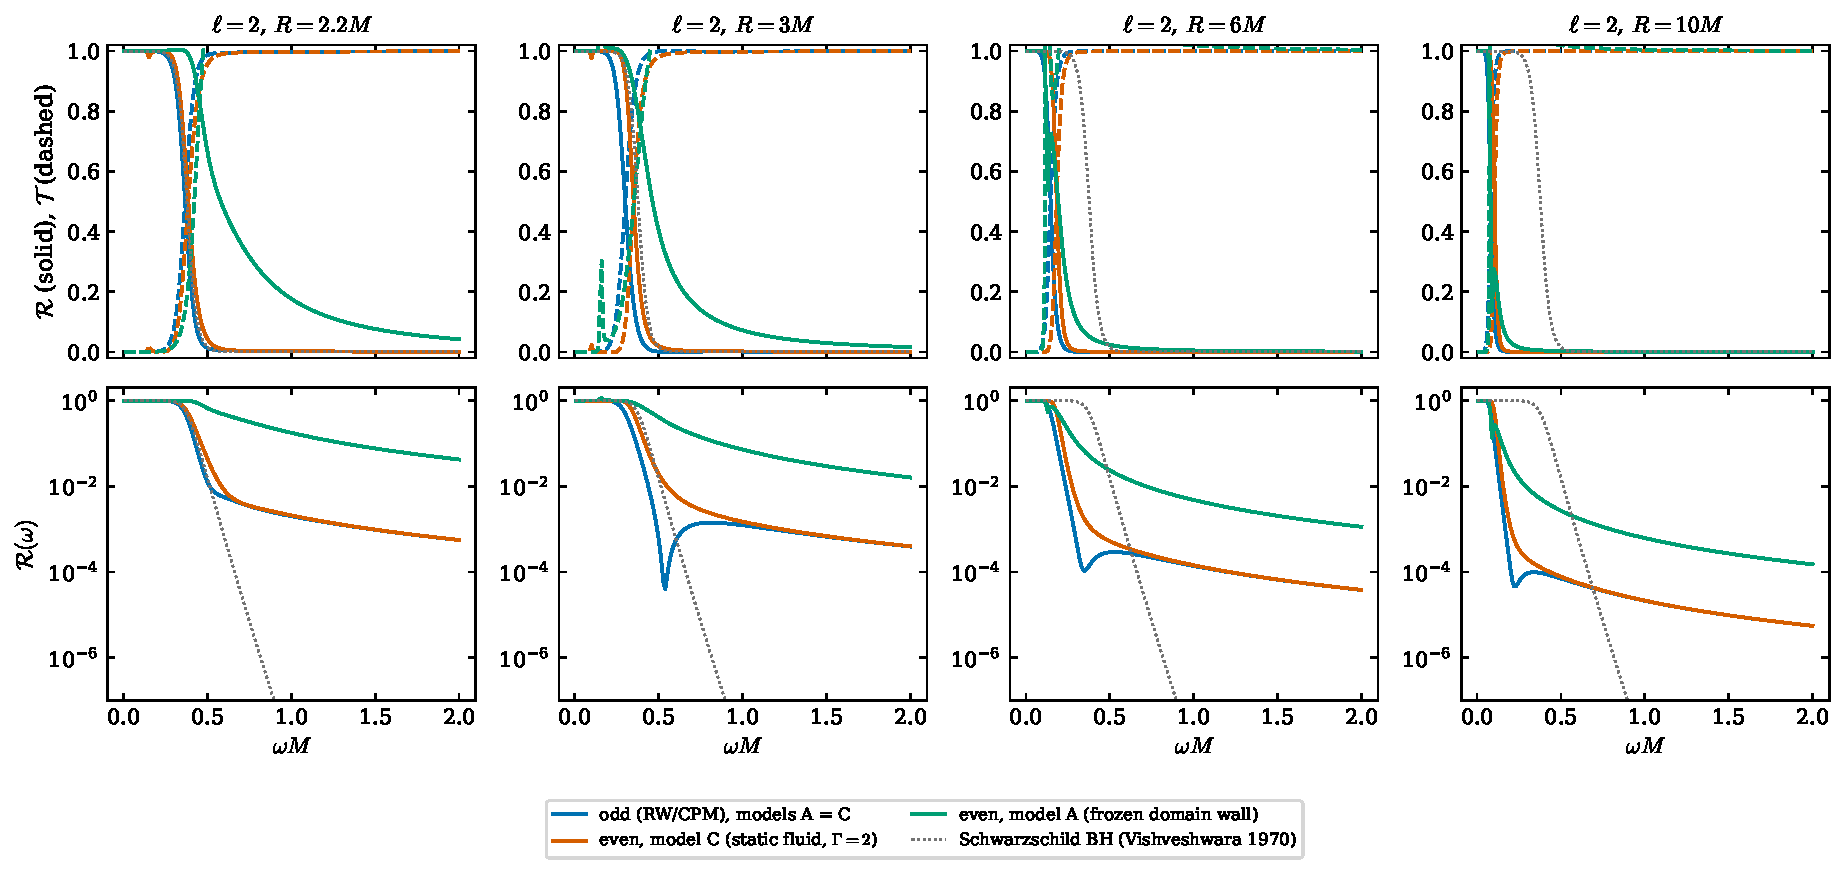
\includegraphics[width=\textwidth]{fig02_RT_l2.pdf}
\caption{Reflection ($\mathcal R$, solid) and transmission ($\mathcal T$, dashed; top row) coefficients,
Eq.~\eqref{eq:RT}, for $\ell=2$ and $R/M=2.2,3,6,10$. Bottom row: $\mathcal R$ on a log scale. Blue: odd
parity (models A and C coincide). Orange: even parity, model C ($\Gamma=2$). Green: even parity, model A.
Grey dotted: Schwarzschild black hole.}\label{fig:RT2}
\end{figure}

\begin{figure}[p]\centering
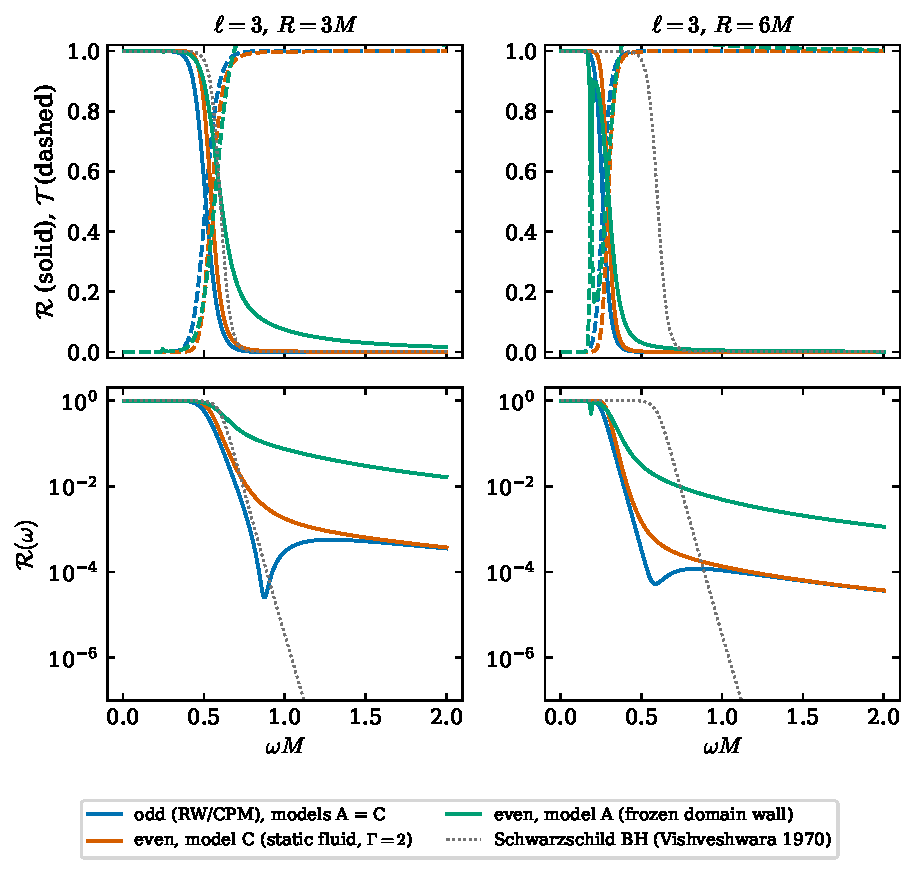
\includegraphics[width=0.8\textwidth]{fig03a_RT_l3.pdf}\\
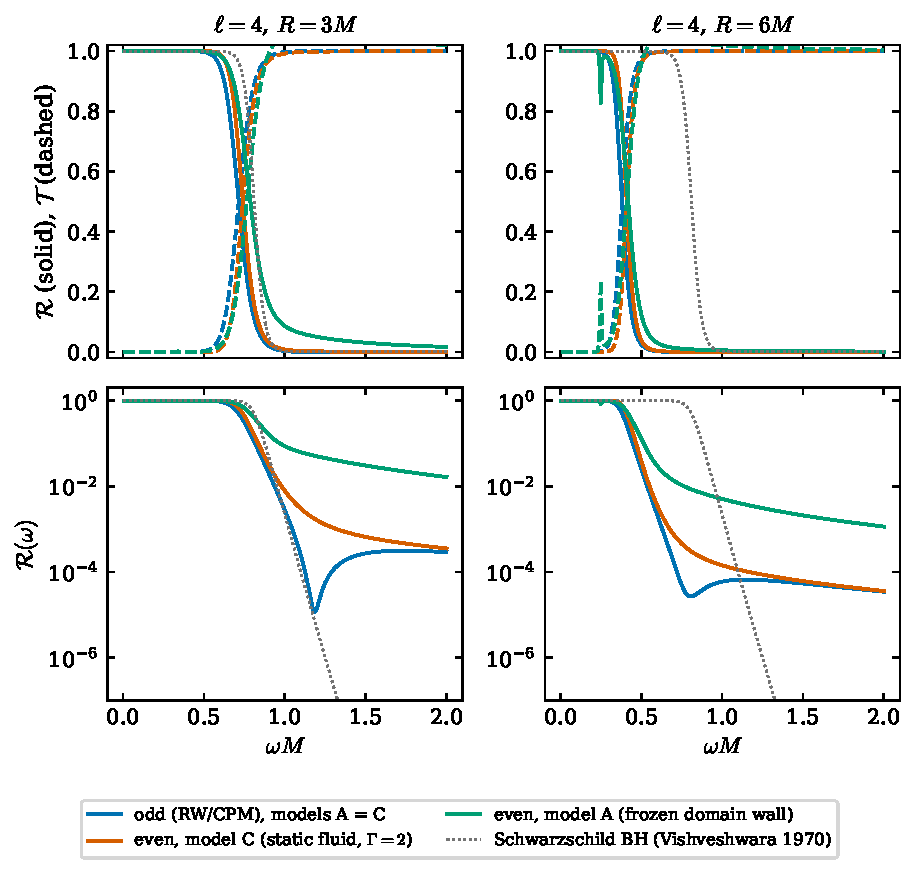
\includegraphics[width=0.8\textwidth]{fig03b_RT_l4.pdf}
\caption{As Fig.~\ref{fig:RT2} for $\ell=3$ (top) and $\ell=4$ (bottom), $R/M=3,6$.}\label{fig:RT34}
\end{figure}

\begin{figure}[t]\centering
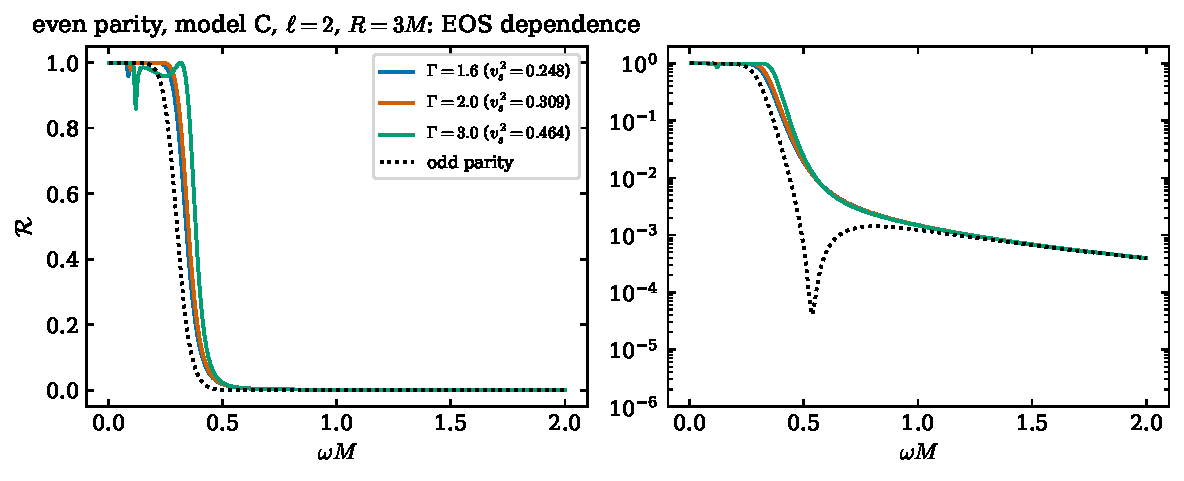
\includegraphics[width=0.85\textwidth]{fig04_eos_dependence.pdf}
\caption{Dependence of the even-parity reflectivity (model C, $\ell=2$, $R=3M$) on the adiabatic index
$\Gamma$ of the shell matter.}\label{fig:eos}
\end{figure}

\begin{figure}[t]\centering
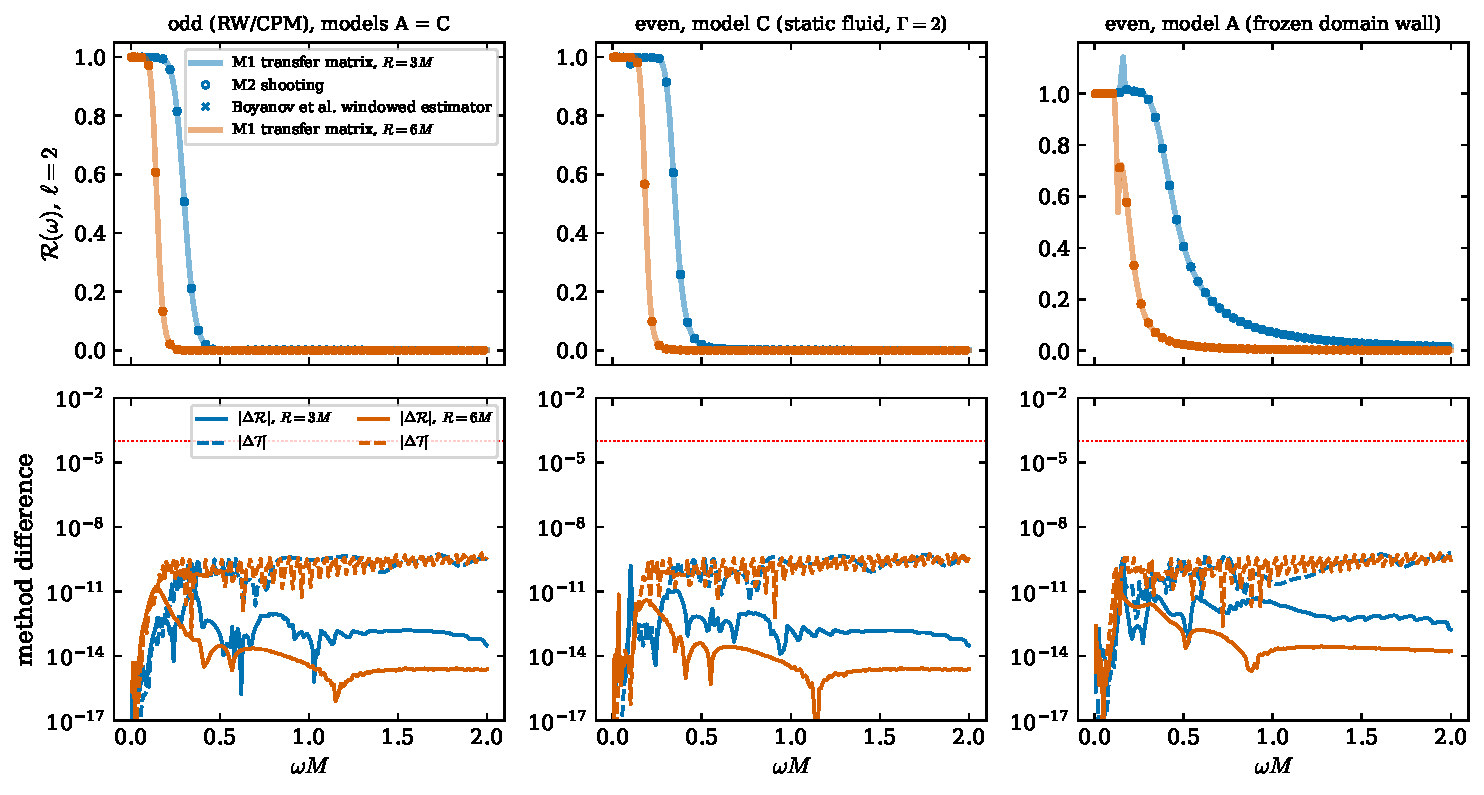
\includegraphics[width=\textwidth]{fig05_transfer_vs_shooting.pdf}
\caption{Transfer matrix (Method 1, lines) vs shooting (Method 2, circles) and the windowed estimator of
Boyanov et al.\ (crosses). The bottom row shows the absolute differences; the red line marks the required
tolerance $10^{-4}$.}\label{fig:tm}
\end{figure}

\begin{figure}[t]\centering
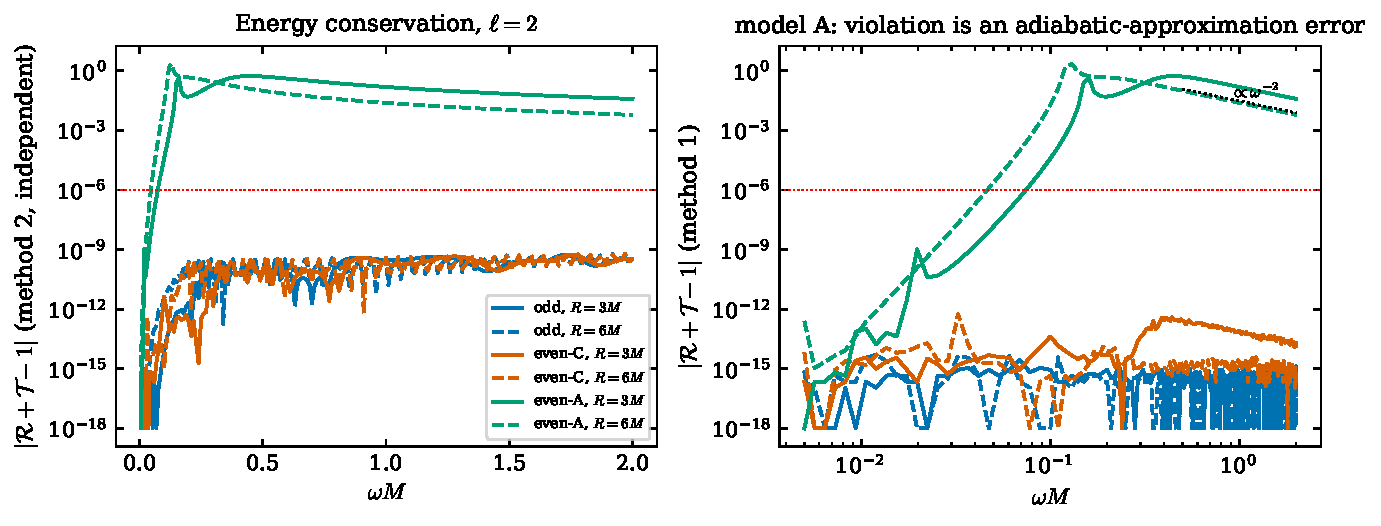
\includegraphics[width=\textwidth]{fig08_energy_conservation.pdf}
\caption{Energy conservation $|\mathcal R+\mathcal T-1|$. Left: Method 2, in which $\mathcal R$ and
$\mathcal T$ are obtained independently from asymptotic amplitudes. Right: Method 1 on log--log axes,
showing that the model-A violation decays as $\omega^{-2}$ (adiabatic error). The red line marks
$10^{-6}$.}\label{fig:energy}
\end{figure}

\begin{figure}[t]\centering
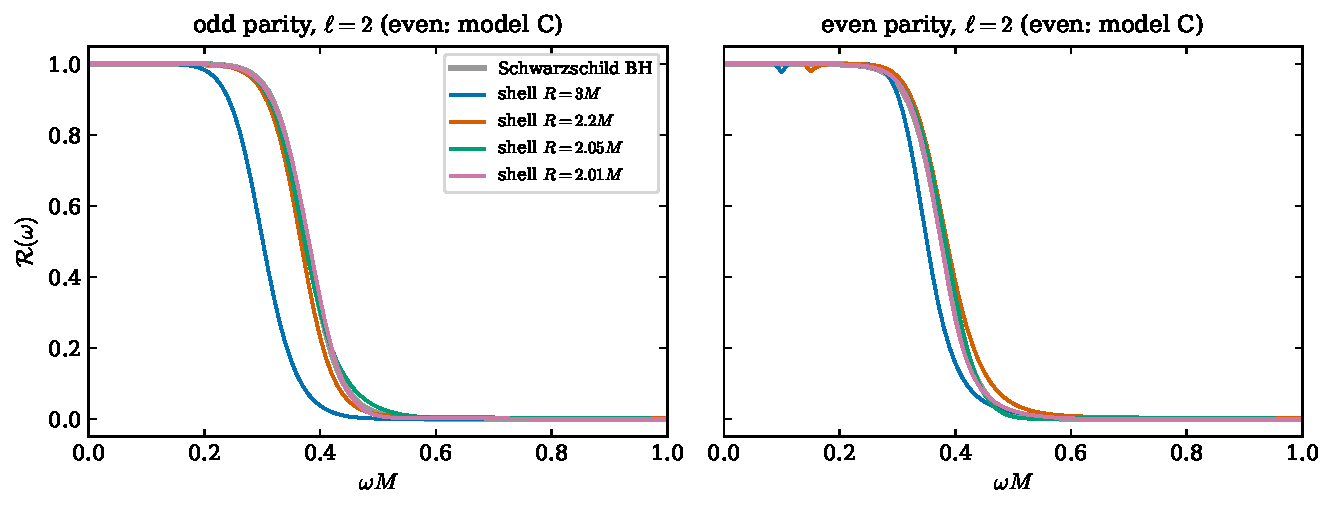
\includegraphics[width=0.9\textwidth]{fig09_schwarzschild_limit.pdf}
\caption{Approach of the shell reflectivity to the Schwarzschild black-hole value (Vishveshwara 1970) as
$R\to2M$.}\label{fig:bhlimit}
\end{figure}

\subsection{Quasinormal modes}\label{sec:res-qnm}
The QNM spectra are shown in Fig.~\ref{fig:qnmplane} (complex plane, shell vs Schwarzschild) and
Fig.~\ref{fig:qnmR} (dependence on $R/M$). Selected values are listed in Tables~\ref{tab:qnm2}--\ref{tab:qnm4}.
The complete list is in \texttt{results/qnm\_table.csv}.
\begin{itemize}
\item \emph{Wave modes} exist in both sectors, with $\omega\sim1/R$. For dilute shells they follow PSP26's
Newtonian law ${\rm Re}(\omega R)\simeq n\pi$ or $(n+\tfrac12)\pi$, ${\rm Im}(\omega R)\simeq-\xi$ with
$\xi=\tfrac12\ln[2\ell(\ell+1)R/M]$ (PSP26 Eqs.~7.23--7.25). The imaginary part grows only logarithmically with
$R/M$: the shell is a weak reflector, and the interior cavity leaks. Quantitatively, our wave modes
coincide with PSP26's exact numerical results (their Figs.~3--4) to the precision with which the figures can
be read ($\pm0.02$); see Table~\ref{tab:psp}.
\item For compact shells ($R<3M$) a family of \emph{trapped} modes appears below the barrier top. Their
damping is set by tunnelling, and as $R\to2M$ they become exponentially long-lived and dense
(Table~\ref{tab:trapped}). They are the modes responsible for GW ``echoes''. None of them tends to the
Schwarzschild QNMs.
\item \emph{Matter modes} (even parity, model C only) are discussed next.
\end{itemize}

\begin{figure}[t]\centering
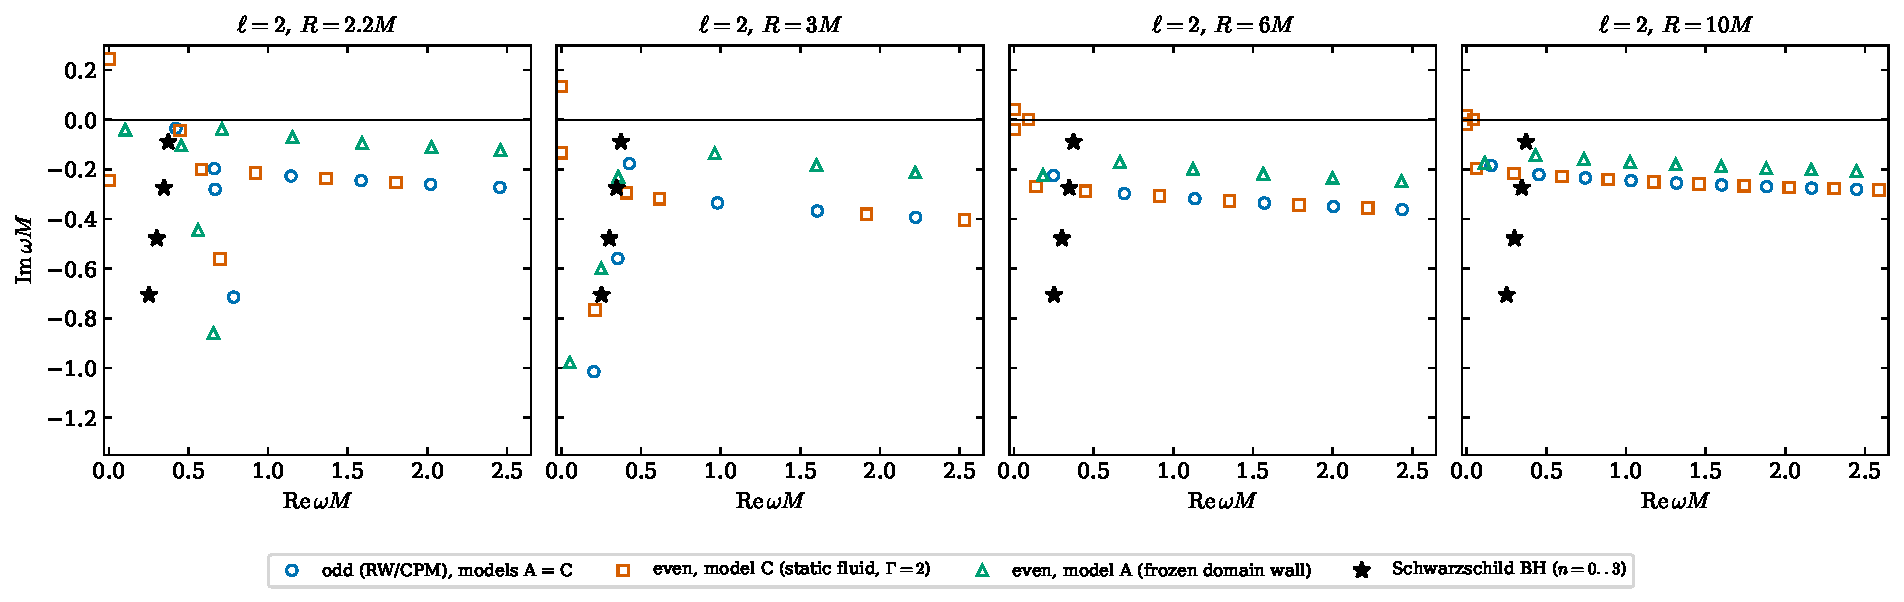
\includegraphics[width=\textwidth]{fig06_qnm_complex_plane.pdf}
\caption{QNMs in the complex $\omega$ plane for $\ell=2$: odd sector (circles), even sector model C (squares),
even sector model A (triangles), and Schwarzschild QNMs (stars). The model-C unstable matter mode lies on the
positive imaginary axis, at $\omega M\approx+i\,0.6(M/R)^{3/2}$.}\label{fig:qnmplane}
\end{figure}

\begin{figure}[t]\centering
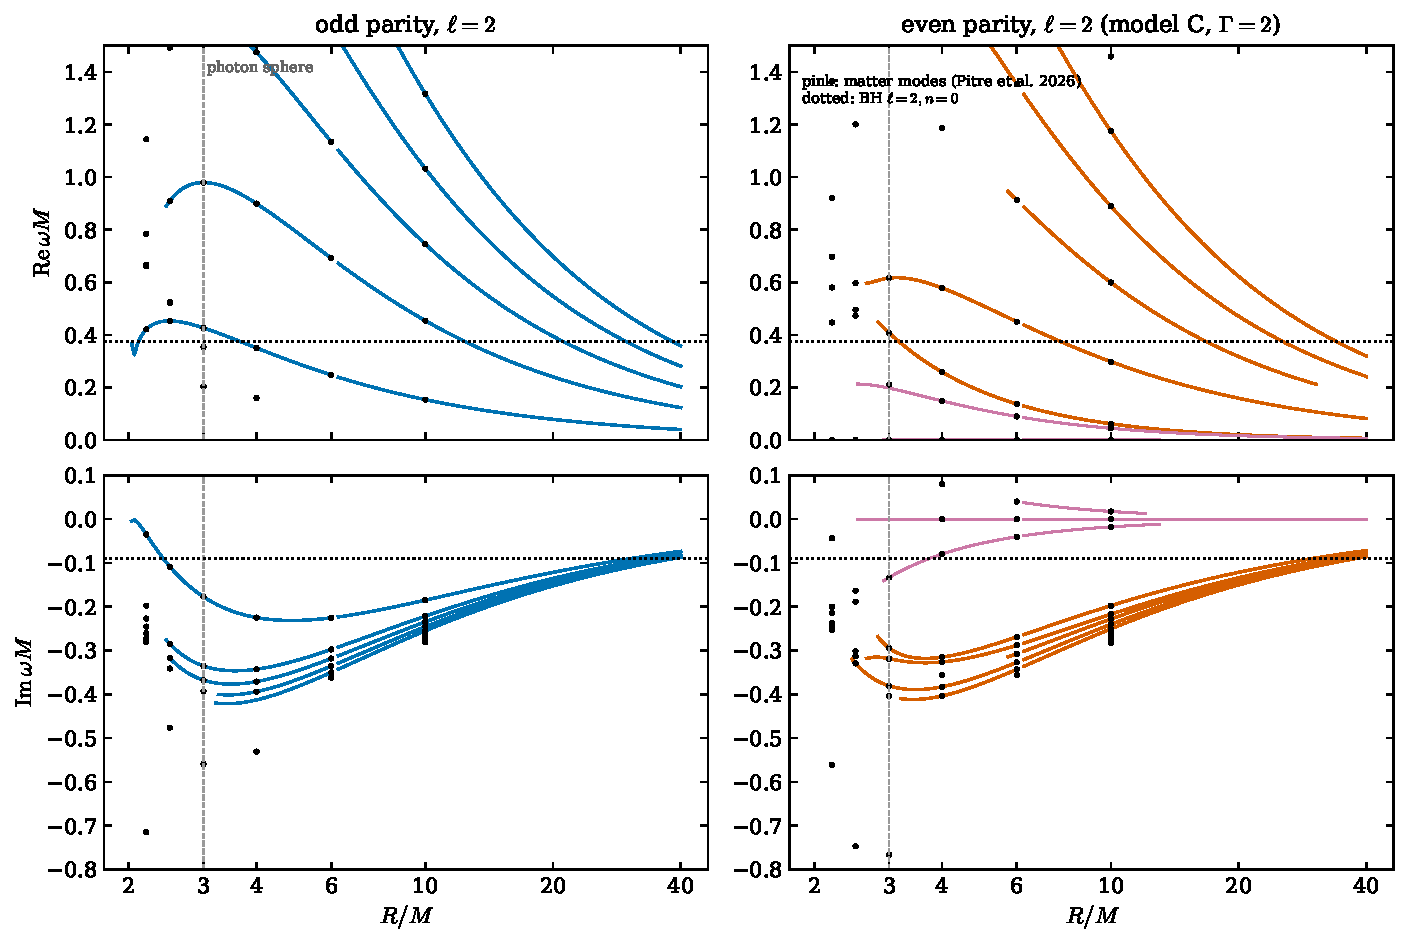
\includegraphics[width=\textwidth]{fig07_qnm_vs_compactness.pdf}
\caption{QNM frequencies vs $R/M$ for $\ell=2$ (continuation in $R$ from the $R=6M$ catalogue; dots are the
independent scans at fixed $R$). The dotted line marks the Schwarzschild $n=0$ mode and the dashed line the
photon sphere $R=3M$.}\label{fig:qnmR}
\end{figure}

\begin{table}[h]\centering\small
\caption{Wave modes ($\ell=2$; even sector: model C, $\Gamma=2$) compared with the values read off PSP26 Figs.~3 and 4 (reading uncertainty $\approx\pm0.02$); $\xi=\tfrac12\ln[2\ell(\ell+1)R/M]$.}\label{tab:psp}
\begin{tabular}{lrrrrrr}\toprule
parity & $M/R$ & mode & ${\rm Re}(R\omega)$ & ${\rm Im}(R\omega)/\xi$ & PSP26 Re & PSP26 Im$/\xi$\\\midrule
odd & 0.167 & 1 & 1.484 & -0.632 & 1.47 & -0.630 \\
odd & 0.167 & 2 & 4.151 & -0.835 & 4.10 & -0.840 \\
even & 0.250 & 1 & 1.033 & -0.651 & 1.05 & -0.655 \\
even & 0.100 & 1 & 0.615 & -0.825 & 0.62 & -0.825 \\
even & 0.100 & 2 & 2.978 & -0.907 & 2.95 & -0.910 \\
\bottomrule\end{tabular}

\end{table}

\begin{table}[h]\centering\scriptsize
\caption{Lowest wave modes, $\ell=2$.}\label{tab:qnm2}
\begin{tabular}{rlp{12cm}}\toprule
$R/M$ & sector & lowest wave modes $\omega M$ (ordered by ${\rm Re}\,\omega$; Methods 1 and 2 agree to $<10^{-4}$)\\\midrule
2.2 & odd & $0.42111-0.03502i$, $0.66196-0.19736i$, $0.66692-0.28043i$, $0.78377-0.71437i$ \\
2.2 & even-C & $0.44694-0.04385i$, $0.57996-0.19970i$, $0.69756-0.56050i$, $0.92055-0.21412i$; matter: $0.00000+0.24429i$, $0.00000-0.24429i$ \\
2.2 & even-A & $0.10284-0.04070i$, $0.45445-0.10428i$, $0.56024-0.44388i$, $0.65595-0.85878i$ \\
3 & odd & $0.20371-1.01489i$, $0.35352-0.55904i$, $0.42638-0.17728i$, $0.97955-0.33508i$ \\
3 & even-C & $0.21102-0.76599i$, $0.40766-0.29425i$, $0.61594-0.31862i$, $1.91546-0.38053i$; matter: $-0.00000+0.13321i$, $-0.00000-0.13326i$ \\
3 & even-A & $0.05288-0.97817i$, $0.24913-0.59916i$, $0.35675-0.22995i$, $0.96224-0.13441i$ \\
6 & odd & $0.24739-0.22534i$, $0.69189-0.29749i$, $1.13482-0.31819i$, $1.57166-0.33553i$ \\
6 & even-C & $0.13710-0.26885i$, $0.45011-0.28793i$, $0.91288-0.30736i$, $1.35361-0.32702i$; matter: $0.08942-0.00005i$, $-0.00000+0.04014i$, $-0.00000-0.04014i$ \\
6 & even-A & $0.18120-0.22393i$, $0.66401-0.17021i$, $1.12337-0.19838i$, $1.56453-0.21844i$ \\
10 & odd & $0.15342-0.18490i$, $0.45405-0.22153i$, $0.74518-0.23457i$, $1.03239-0.24567i$ \\
10 & even-C & $0.06152-0.19748i$, $0.29784-0.21714i$, $0.59930-0.22783i$, $0.88902-0.24022i$; matter: $0.04421-0.00001i$, $-0.00000+0.01762i$, $0.00000-0.01762i$ \\
10 & even-A & $0.11383-0.17403i$, $0.43293-0.14212i$, $0.73603-0.15791i$, $1.02659-0.17041i$ \\
\bottomrule\end{tabular}

\end{table}
\begin{table}[h]\centering\scriptsize
\caption{Lowest wave modes, $\ell=3$.}\label{tab:qnm3}
\begin{tabular}{rlp{12cm}}\toprule
$R/M$ & sector & lowest wave modes $\omega M$ (ordered by ${\rm Re}\,\omega$; Methods 1 and 2 agree to $<10^{-4}$)\\\midrule
2.2 & odd & $0.61197-0.01610i$, $0.79559-0.14940i$, $0.92563-0.26191i$, $1.32591-0.24723i$ \\
2.2 & even-C & $0.62406-0.01797i$, $0.94668-0.42655i$, $1.05770-0.83502i$, $1.09205-0.23717i$; matter: $0.00000+0.33715i$, $0.00000-0.33715i$ \\
2.2 & even-A & $0.66172-0.05295i$, $0.80201-0.33708i$, $0.86783-0.05466i$, $0.90221-0.70492i$ \\
3 & odd & $0.45895-0.96508i$, $0.60569-0.55699i$, $0.65509-0.18820i$, $1.22298-0.38277i$ \\
3 & even-C & $0.35057-1.17392i$, $0.54273-0.73309i$, $0.66906-0.23954i$, $0.83640-0.42456i$; matter: $0.31096-0.00003i$, $0.00000+0.22263i$, $-0.00000-0.22263i$ \\
3 & even-A & $0.36818-0.96443i$, $0.52224-0.58563i$, $0.61501-0.22237i$, $1.18558-0.16840i$ \\
6 & odd & $0.19277-0.46109i$, $0.40294-0.26528i$, $0.86444-0.33236i$, $1.31485-0.33882i$ \\
6 & even-C & $0.05982-0.50984i$, $0.33182-0.32097i$, $0.59758-0.34764i$, $1.08605-0.33206i$; matter: $0.13334-0.00000i$, $0.00000+0.07705i$, $-0.00000-0.07705i$ \\
6 & even-A & $0.15669-0.44150i$, $0.35437-0.25459i$, $0.82650-0.19835i$, $1.30131-0.21402i$ \\
10 & odd & $0.07849-0.31820i$, $0.25779-0.21802i$, $0.56823-0.24477i$, $0.86393-0.24851i$ \\
10 & even-C & $0.18733-0.24644i$, $0.39972-0.25566i$, $0.71377-0.24471i$, $1.00967-0.25121i$; matter: $0.06489-0.00000i$, $-0.00000+0.03530i$, $0.00000-0.03530i$ \\
10 & even-A & $0.06376-0.29784i$, $0.22599-0.20104i$, $0.54149-0.16173i$, $0.85350-0.16877i$ \\
\bottomrule\end{tabular}

\end{table}
\begin{table}[h]\centering\scriptsize
\caption{Lowest wave modes, $\ell=4$.}\label{tab:qnm4}
\begin{tabular}{rlp{12cm}}\toprule
$R/M$ & sector & lowest wave modes $\omega M$ (ordered by ${\rm Re}\,\omega$; Methods 1 and 2 agree to $<10^{-4}$)\\\midrule
2.2 & odd & $0.78350-0.00632i$, $0.96055-0.10943i$, $1.12058-0.23837i$, $1.21974-0.52330i$ \\
2.2 & even-C & $0.79313-0.00713i$, $0.95445-0.10853i$, $1.25457-0.26967i$, $1.72821-0.26728i$; matter: $1.27806-0.72384i$ \\
2.2 & even-A & $0.84021-0.02540i$, $1.01805-0.27016i$, $1.02364-0.06398i$, $1.95769-0.11146i$ \\
3 & odd & $0.83612-0.55496i$, $0.86734-0.19128i$, $1.46401-0.42352i$, $2.10831-0.42242i$ \\
3 & even-C & $0.62773-1.12565i$, $0.81795-0.71396i$, $0.87869-0.22137i$, $1.05472-0.49667i$; matter: $0.42113-0.00000i$, $0.00000+0.30830i$, $0.00000-0.30830i$ \\
3 & even-A & $0.76236-0.57809i$, $0.83678-0.22130i$, $1.40641-0.19861i$, $2.09450-0.22031i$ \\
6 & odd & $0.11490-0.66203i$, $0.34725-0.50399i$, $0.55217-0.29359i$, $1.03466-0.36255i$ \\
6 & even-C & $0.24097-0.55312i$, $0.50342-0.35230i$, $0.74190-0.40586i$, $1.25433-0.35402i$; matter: $0.17772-0.00000i$, $-0.00000+0.11153i$, $-0.00000-0.11153i$ \\
6 & even-A & $0.08922-0.62756i$, $0.30788-0.47992i$, $0.50763-0.28112i$, $0.98618-0.22296i$ \\
10 & odd & $0.18066-0.35695i$, $0.35821-0.24238i$, $0.68050-0.26493i$, $0.97986-0.26164i$ \\
10 & even-C & $0.09507-0.37186i$, $0.30022-0.27956i$, $0.49865-0.29120i$, $0.82490-0.25981i$; matter: $0.08609-0.00000i$, $-0.00000+0.05180i$, $-0.00000-0.05180i$ \\
10 & even-A & $0.16134-0.33379i$, $0.32745-0.22396i$, $0.64779-0.17880i$, $0.96788-0.17874i$ \\
\bottomrule\end{tabular}

\end{table}
\begin{table}[h]\centering\small
\caption{Trapped modes of ultracompact shells (odd, $\ell=2$): exact vs WKB.}\label{tab:trapped}
\begin{tabular}{rll}\toprule
$R/M$ & exact (M1) & WKB (Bohr--Sommerfeld + Gamow)\\\midrule
2.01 & $0.162603-9.711e-07\,i$ & $0.152432-5.081e-07\,i$ \\
2.01 & $0.248683-5.284e-05\,i$ & $0.246194-3.249e-05\,i$ \\
2.01 & $0.326133-8.798e-04\,i$ & $0.328792-7.287e-04\,i$ \\
2.02 & $0.216610-1.809e-05\,i$ & $0.205905-8.922e-06\,i$ \\
2.02 & $0.322125-1.072e-03\,i$ & $0.324183-8.289e-04\,i$ \\
2.05 & $0.302815-8.384e-04\,i$ & $0.296095-4.811e-04\,i$ \\
2.10 & $0.367989-8.195e-03\,i$ & $0.370495-7.304e-03\,i$ \\
\bottomrule\end{tabular}

\end{table}

\subsection{Even-parity matter modes and the instability of the static shell}\label{sec:res-matter}
The literature search (Sec.~\ref{sec:refs}) found that our system, the static perfect-fluid shell with
Minkowski interior and Schwarzschild exterior, has been studied very recently by Pitre, Schneider \& Poisson
[PSP26, arXiv:2604.05980]. They found four even-parity ``matter modes'' per $\ell$: an unstable purely
imaginary one, its damped mirror, and a pair $\pm{\rm Re}\,\omega+i\,{\rm Im}\,\omega$ with small
negative imaginary part. They concluded that the shell is dynamically unstable on all angular scales. Their
method is different from ours: retarded-time slicing, an RW-type master function in both sectors, and
Chebyshev collocation / MST. We therefore reproduce their results as an independent validation of our
even-parity junction conditions (Table~\ref{tab:pitre}, Fig.~\ref{fig:pitre}).
\begin{itemize}
\item At $M/R=0.2$, $\Gamma=2$, $\ell=2$ we find $\omega(R^3/M)^{1/2}=0.60771\,i$ for the unstable mode and
$1.26707-0.00110\,i$ for the stable pair. These agree with PSP26 Figs.~1 and 2, which show $\approx0.61\,i$
and $\approx1.27-1.1\times10^{-3}i$.
\item As $M/R\to0$ our values approach the post-Newtonian limits of PSP26 Eq.~(7.8), $0.51470\,i$ and
$1.50496$. At $M/R=0.01$ the differences are $0.0040$ and $0.0098$, of the size of the expected $O(M/R)$
correction.
\end{itemize}
This settles the question raised in Sec.~\ref{sec:choice}. The truly static model C is linearly unstable,
with growth time $\sim1.6(R^3/M)^{1/2}$. This is comparable to the collapse time of the domain wall of
model A. Neither background is stable on the dynamical timescale. The real-frequency scattering results are
valid in the high-frequency regime stated at the beginning of this document.

\begin{table}[h]\centering\small
\caption{Even-parity matter modes, model C, $\ell=2$, $\Gamma=2$. $|\Delta_{12}|$ is the difference
between Methods 1 and 2. Compare PSP26 Figs.~1--2 and their Eq.~(7.8).}\label{tab:pitre}
\begin{tabular}{rllll}\toprule
$M/R$ & unstable: $\omega(R^3/M)^{1/2}$ & $|\Delta_{12}|$ & stable pair: $\omega(R^3/M)^{1/2}$ & $|\Delta_{12}|$\\\midrule
0.30 & $0.668693\,i$ & 1.6e-12 & $1.095903-1.70e-03\,i$ & 1.8e-12 \\
0.25 & $0.636634\,i$ & 7.1e-12 & $1.188088-1.51e-03\,i$ & 9.2e-13 \\
0.20 & $0.607709\,i$ & 1.6e-11 & $1.267067-1.10e-03\,i$ & 3.9e-13 \\
0.15 & $0.581398\,i$ & 2.3e-11 & $1.336362-6.47e-04\,i$ & 5.1e-13 \\
0.10 & $0.557313\,i$ & 3.3e-11 & $1.398197-2.78e-04\,i$ & 6.1e-13 \\
0.05 & $0.535158\,i$ & 4.6e-11 & $1.454057-5.79e-05\,i$ & 7.4e-13 \\
0.02 & $0.522690\,i$ & 4.6e-11 & $1.485144-6.52e-06\,i$ & 8.3e-13 \\
0.01 & $0.518662\,i$ & 6.1e-11 & $1.495140-1.20e-06\,i$ & 0.0e+00 \\
$\to0$ (PN, PSP26 Eq.~7.8) & $0.514695\,i$ & & $1.504962$ & \\
\bottomrule\end{tabular}

\end{table}

\begin{figure}[t]\centering
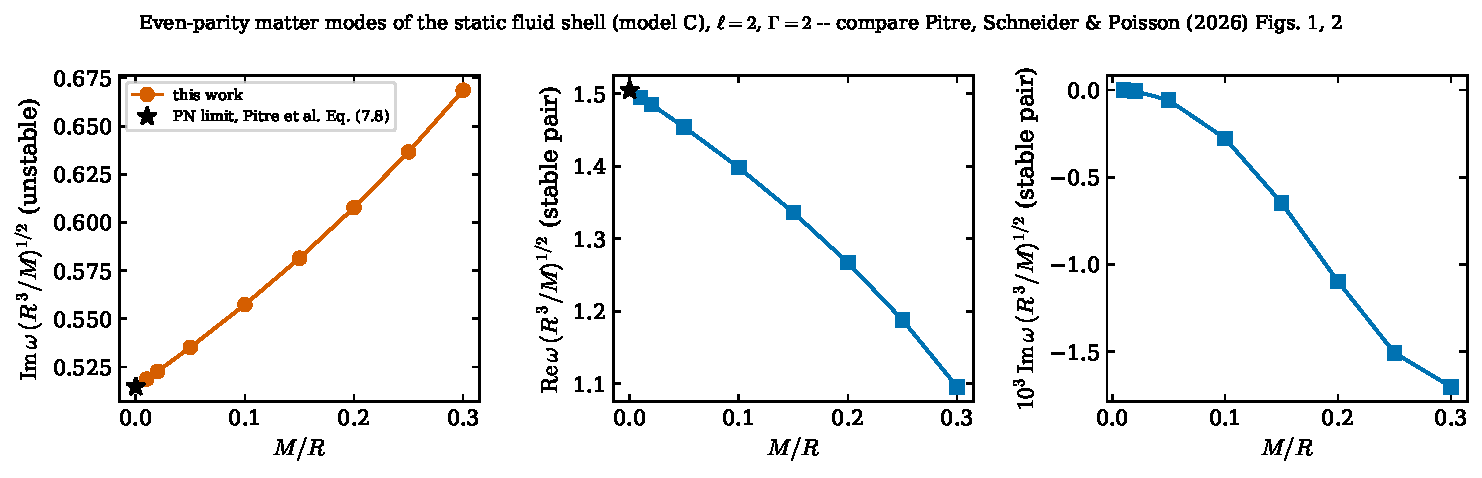
\includegraphics[width=\textwidth]{fig10_matter_modes_pitre.pdf}
\caption{Matter modes of the static fluid shell vs compactness, with the post-Newtonian limits of PSP26
(stars).}\label{fig:pitre}
\end{figure}

\begin{figure}[t]\centering
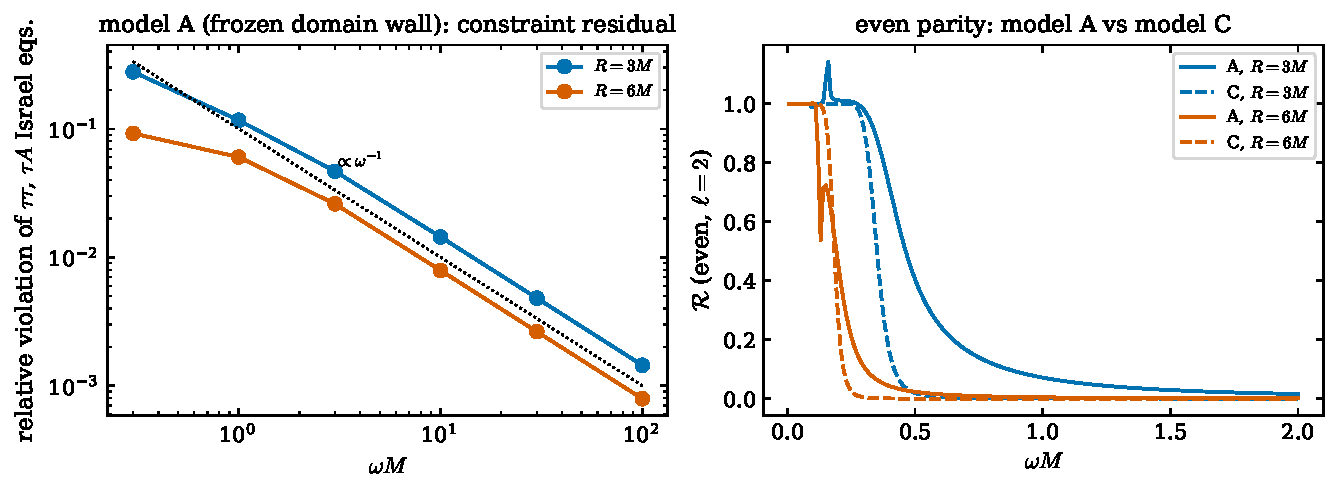
\includegraphics[width=0.95\textwidth]{fig11_modelA_adiabatic.pdf}
\caption{Model A (frozen domain wall). Left: relative violation of the $\tau\tau$ and $\tau A$ Israel
constraints, $\propto\omega^{-1}$. Right: even-parity reflectivity of models A and C.}\label{fig:modelA}
\end{figure}

\begin{figure}[t]\centering
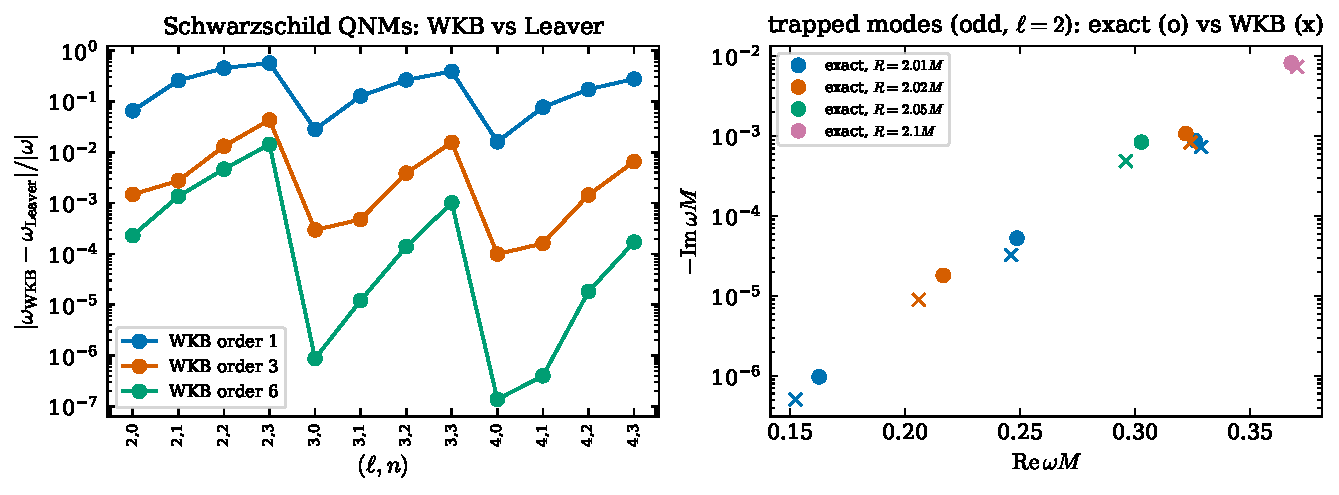
\includegraphics[width=0.95\textwidth]{fig12_wkb.pdf}
\caption{WKB validation. Left: Schwarzschild QNMs at WKB orders 1, 3 and 6 vs Leaver. Right: trapped modes
of ultracompact shells, exact (o) vs WKB (x).}\label{fig:wkb}
\end{figure}

%======================================================================
\section{Discussion}\label{sec:disc}
\begin{enumerate}
\item \textbf{Shell model.} No static configuration exists for a pure domain wall or a dust shell. A static
shell needs positive surface pressure, $p/\sigma=(1-\sq)/(4\sq)$. Even that shell is dynamically unstable
(PSP26, confirmed here). The ``collapse problem'' of the prior notes is therefore generic: every thin shell
of this type evolves on the timescale $(R^3/M)^{1/2}$. GW scattering in the frequency domain is an adiabatic
concept, valid for $\omega(R^3/M)^{1/2}\gg1$. We quantified the accuracy of the adiabatic domain-wall model,
and found it to be $O(\omega_{\rm dyn}/\omega)$.
\item \textbf{Junction conditions.} Odd parity: $[\Psi]=0$ and $[\partial_x\Psi]=\Delta_{\rm odd}\Psi$, with
$\Delta_{\rm odd}=\sq(1-\sq)/R$, independent of $\omega$ and of the equation of state. The $[K]^{(0)}$ term that
worried the prior notes cancels against $\delta S_{\tau A}$. Even parity: a frequency-dependent $2\times2$
matrix. The radial displacement of the shell differs between the two RW gauges, and the shell's
compressional dynamics enter through $v_s^2$.
\item \textbf{Relation to previous work.} Our odd junction agrees with PSP26 and with Pani et al.\ (2009).
Our even junction reproduces PSP26's matter modes. Pani et al.'s gravastar has $\Sigma=0$ and a de Sitter
interior, so no direct numerical comparison is possible; we did check agreement of the structural matching
conditions. PSP26 argue that unstable modes should also exist in Pani et al.'s model.
\item \textbf{What is new here} relative to PSP26:
\begin{itemize}
\item the reflection and transmission coefficients $\mathcal R$ and $\mathcal T$, with their low-frequency,
high-frequency and black-hole limits;
\item the explicit $\delta$-function form of the odd junction;
\item the adiabatic domain-wall model and the quantification of its error;
\item two independent numerical methods agreeing to $\lesssim10^{-8}$.
\end{itemize}
\item \textbf{Limitations.}
\begin{itemize}
\item Model C is restricted to $R\ge2.1M$ by the energy and causality conditions.
\item The frozen-wall QNMs are meaningful only for $|\omega|\gg\omega_{\rm dyn}$.
\item Like PSP26, we do not attempt a time-domain evolution of the unstable shell.
\end{itemize}
\end{enumerate}


%======================================================================
\section{References and equation map}\label{sec:refs}
\begin{description}\small
\item[{[RW57]}] T.~Regge and J.~A.~Wheeler, \emph{Stability of a Schwarzschild singularity}, Phys.\ Rev.\ \textbf{108},
  1063 (1957). Used: Eq.~(25) (odd potential), Eqs.~(18), (20) (RW gauge).
\item[{[Z70]}] F.~J.~Zerilli, \emph{Effective potential for even-parity Regge--Wheeler gravitational perturbation
  equations}, Phys.\ Rev.\ Lett.\ \textbf{24}, 737 (1970). Used: first-order system and algebraic identity
  (p.~737), Eq.~(3) ($r_*$), Eq.~(5) ($V_{\rm Z}$).
\item[{[V70]}] C.~V.~Vishveshwara, \emph{Scattering of gravitational radiation by a Schwarzschild black-hole},
  Nature \textbf{227}, 936 (1970). Used: Fig.~2 ($\mathcal R$ vs $k^2=(2M\omega)^2$, $\ell=2$ odd) as a check.
\item[{[MP05]}] K.~Martel and E.~Poisson, \emph{Gravitational perturbations of the Schwarzschild spacetime: a practical
  covariant and gauge-invariant formalism}, Phys.\ Rev.\ D \textbf{71}, 104003 (2005). Used: Eqs.~(3.1)--(3.7)
  (harmonics), (4.1)--(4.3), (4.23)--(4.26) (even), (5.1)--(5.3), (5.7)--(5.9), (5.13)--(5.18) (odd).
  K.~Martel, PhD thesis (Guelph 2004): derivations behind MP05 (consulted).
\item[{[IS84]}] J.~Ipser and P.~Sikivie, \emph{Gravitationally repulsive domain wall}, Phys.\ Rev.\ D \textbf{30}, 712
  (1984). Used: Eqs.~(2.1)--(2.3), (2.6), (2.8), (2.9)--(2.12), (3.1)--(3.9).
\item[{[P04]}] E.~Poisson, \emph{A Relativist's Toolkit} (Cambridge 2004). Used: Eqs.~(3.49), (3.56) (junction
  conditions), (3.65), (3.68)--(3.70) (thin-shell collapse), (3.75)--(3.81) (static shell: interior time
  normalization, $\sigma$, $p$).
\item[{[AS72]}] M.~Abramowitz and I.~A.~Stegun, \emph{Handbook of Mathematical Functions} (1972), Sec.~10.3; DLMF
  Ch.~10 (Riccati--Bessel functions, Wronskian 10.50.1).
\item[{[PBCCN09]}] P.~Pani, E.~Berti, V.~Cardoso, Y.~Chen and R.~Norte, \emph{Gravitational wave signatures of the absence
  of an event horizon: nonradial oscillations of a thin-shell gravastar}, Phys.\ Rev.\ D \textbf{80}, 124047
  (2009), arXiv:0909.0287. Used: Eqs.~(3.29), (3.33), (A16), (A20), (A35) (junction structure; comparison),
  App.~B Eqs.~(B3)--(B19) (continued fraction about $R_2$, adapted to $e^{-i\omega t}$), Sec.~III.B (Chandrasekhar map).
\item[{[PSP26]}] T.~Pitre, B.~Schneider and E.~Poisson, \emph{Self-gravitating thin shells are dynamically unstable on
  all angular scales}, arXiv:2604.05980 [gr-qc] (2026). \textbf{Same physical system as our model C}. Used:
  Eqs.~(1.1)--(1.2), (2.4)--(2.6) (polytropic shell, $\Gamma$), (5.23)/(97) (odd junction: agreement), (7.8)
  (post-Newtonian matter modes), (7.23)--(7.25) (Newtonian wave modes), Figs.~1--4 (quantitative comparison).
\item[{[BCKR24]}] V.~Boyanov, V.~Cardoso, K.~D.~Kokkotas and J.~Redondo-Yuste, \emph{The dynamical response of viscous
  objects to gravitational waves}, arXiv:2411.16861, Phys.\ Rev.\ Lett.\ \textbf{135}, 151402 (2025). This paper
  was not in \texttt{Bibliography/}; it was retrieved from arXiv. Used: Eq.~(15) (conventions), Eq.~(17)
  (reflectivity), App.~B1 (windowed estimator $|i\omega+\psi'/\psi|/|i\omega-\psi'/\psi|$; inward integration
  from a high-order exterior expansion for QNMs), Eq.~(14) and inviscid limit (continuity of $\psi$, $\psi'$),
  Fig.~1 (low-frequency $\mathcal R^2\to1$).
\item[{[L85]}] E.~W.~Leaver, Proc.\ R.\ Soc.\ Lond.\ A \textbf{402}, 285 (1985) (continued fraction, Eqs.~5--8 and
  inversion). [BCS09] E.~Berti, V.~Cardoso and A.~O.~Starinets, Class.\ Quantum Grav.\ \textbf{26}, 163001 (2009)
  (QNM tables). [LNS93] M.~Leins, H.-P.~Nollert and M.~H.~Soffel, Phys.\ Rev.\ D \textbf{48}, 3467 (1993).
\item[{[SW85, IW87, K03]}] B.~F.~Schutz and C.~M.~Will, Astrophys.\ J.\ Lett.\ \textbf{291}, L33 (1985);
  S.~Iyer and C.~M.~Will, Phys.\ Rev.\ D \textbf{35}, 3621 (1987) (Eq.~1.5, Table~I); R.~A.~Konoplya, Phys.\ Rev.\ D
  \textbf{68}, 024018 (2003). Y.~Hatsuda, Phys.\ Rev.\ D \textbf{101}, 024008 (2020) (WKB = Bender--Wu series).
  J.~Killingbeck, Phys.\ Lett.\ A \textbf{65}, 87 (1978) (hypervirial perturbation method).
\item[{[C83]}] S.~Chandrasekhar, \emph{The Mathematical Theory of Black Holes} (Oxford 1983), Sec.~4.26.
\item[{Other}] V.~Cardoso, E.~Franzin and P.~Pani, Phys.\ Rev.\ Lett.\ \textbf{116}, 171101 (2016) (echoes of
  ultracompact objects). H.~Yang, B.~Bonga and U.-L.~Pen (cited in PSP26; eikonal instability of thin shells).
  Prior notes: \texttt{Starting point/interior\_ondas\_cascara.pdf} and \texttt{burbuja\_matching\_israel.pdf}.
\end{description}

\paragraph{Honesty statement.} A literature search (arXiv/Google Scholar, queries ``thin shell
quasinormal modes Minkowski interior'', ``thin-shell gravastar perturbations'') found that the QNM spectrum
of our model C has been computed by PSP26. We reproduce their matter and wave modes and cite them as a
validation, not as a new result. We found no published reflection/transmission coefficients for this
system.

\paragraph{Corrections to the starting documents and to the task statement.}
\begin{enumerate}
\item The regular interior solution is $\jh(\nu r)$ with $\nu=\omega/\sq$, not $\jh(\omega r)$, when $\omega$
  is the exterior Killing frequency (Sec.~\ref{sec:blueshift}).
\item A static dust shell (``Option B'') does not exist. The formula $M=4\pi\sigma R^2\sqrt f$ is incorrect
  (Sec.~\ref{sec:choice}).
\item The background-trace term $[K]^{(0)}$ of \texttt{burbuja\_matching\_israel} Eq.~(13) cancels against the
  pressure term of $\delta S_{\tau A}$ (Sec.~\ref{sec:odd}). The $\ddot R$ dependence therefore drops out of the
  odd sector exactly. In the even sector it survives, but model A must then be treated as an
  $O(\omega_{\rm dyn}/\omega)$ approximation.
\item Pure-Schwarzschild QNMs are not a limit of the shell spectrum. The $\ell=2$, $n=0$ value is reproduced by
  our exterior solver with black-hole boundary conditions, and $\mathcal R(\omega)$ tends to the black-hole value
  as $R\to2M$, but the shell QNMs do not (Sec.~\ref{sec:res-valid}).
\end{enumerate}

\appendix
\section{Code map}
{\small\begin{tabular}{p{6.3cm}p{9.3cm}}
\texttt{code/main.py} & driver: \texttt{validate, scatter, qnm, tracks, csv, figures}\\
\texttt{code/symbolic/vacuum\_relations.py} & Einstein-tensor linearization; Eqs.~\eqref{eq:oddrecon}, \eqref{eq:Krec}--\eqref{eq:Hrec}\\
\texttt{code/symbolic/derive\_junction.py} & first-principles junction conditions; exports $\mathsf A$, $\mathsf B$\\
\texttt{code/symbolic/exterior\_series.py} & continued-fraction recurrence; Chandrasekhar map\\
\texttt{code/shellgw/background.py} & shell models (Sec.~\ref{sec:bg})\\
\texttt{code/shellgw/interior.py}, \texttt{exterior.py} & interior functions; exterior ODE, asymptotic series, continued fraction\\
\texttt{code/shellgw/junction.py} & transfer matrices (odd analytic; even generated; mpmath near $2M$)\\
\texttt{code/shellgw/scattering.py}, \texttt{qnm.py} & Methods 1 and 2 for $\mathcal R$, $\mathcal T$ and QNMs\\
\texttt{code/shellgw/blackhole.py}, \texttt{wkb.py} & Leaver; arbitrary-order WKB; trapped-mode WKB\\
\texttt{results/} & JSON results, \texttt{qnm\_table.csv}, logs\\
\texttt{figures/} & all figures (PDF and PNG)
\end{tabular}}

\end{document}
